\documentclass[12pt, twoside]{article}
\usepackage[utf8]{inputenc}
\usepackage[english]{babel}

\usepackage{amsthm}
\usepackage{a4wide}
\usepackage{graphicx}
\usepackage{caption}
\usepackage{amssymb}
\usepackage{amsmath}
\usepackage{mathrsfs}
\usepackage{euscript}
\usepackage{graphicx}
\usepackage{subfig}
\usepackage{caption}
\usepackage{color}
\usepackage{bm}
\usepackage{tabularx}
\usepackage{adjustbox}


\usepackage[toc,page]{appendix}

\usepackage{comment}
\usepackage{rotating}

\DeclareMathOperator*{\argmax}{arg\,max}
\DeclareMathOperator*{\argmin}{arg\,min}

\newtheorem{theorem}{Theorem}
\newtheorem{lemma}[theorem]{Lemma}
\newtheorem{definition}{Definition}[section]

%\numberwithin{equation}{section}

\newcommand*{\No}{No.}

\usepackage{autonum}

\begin{document}

\title{\bf Prior distribution choices for a mixture of experts \thanks{This research was supported by RFBR (project ???) and NTI (project ???).}}
\date{}
\author{}
\maketitle

\begin{center}
\bf
A. V. Grabovoy\footnote{Moscow Institute of Physics and Technology, grabovoy.av@phystech.edu},
V. V. Strijov\footnote{Moscow Institute of Physics and Technology, Dorodnicyn Computing Centre, Federal Research Center “Computer Science and Control” of the Russian Academy of Sciences, strijov@phystech.edu}
\end{center}
{\centering\begin{quote}
\textbf{Abstract:} 
The paper investigates a mixture of expert models. 
The mixture of experts is a set of experts and the gate function which weighs these experts. Each expert is a linear model.
The gate function is a neural network with softmax on the last layer. 
The paper analyzes different prior distributions for each expert.
The authors propose a method that takes into account the relationship between the prior distributions of different experts.
The paper uses the EM algorithm for solving the optimization problem.
This paper proposes to use the mixture of experts for the problem of circles parameters estimation.
Each expert fits one circle in the image.
The experiment uses synthetic and real data to test the proposed method.
The real data is a human eye image from the iris detection problem.


\smallskip
\textbf{Keywords}: mixture of Experts; bayesian model selection; prior distribution.

\smallskip
\end{quote}
}

\section{Introduction}
The paper studies the problem of a mixture of experts constructing. A mixture of experts is multimodel, which are weighed local models that approximate the dataset. The weighting coefficients depend on datum from the dataset.

Examples of multimodel are bagging, gradient boosting~\cite{Tianqi2016} and random forest~\cite{Ishwaran2012}. There are approaches to multimodeling~\cite{Yuksel2012} suggests that the contribution of each expert to the answer depends on the object from the dataset. A mixture of experts uses a gate function that weights the prediction of each expert.

The main problem of multimodal is a convergence dependence on the initial point.
We are using the probability approach for finding optimal mixture parameters and local expert parameters.
The paper proposes to use different prior distribution on parameters to improve convergence.
The paper introduces the method which is using a dependence between prior distribution to improve multimodel quality.

\begin{figure}[h!t]\center
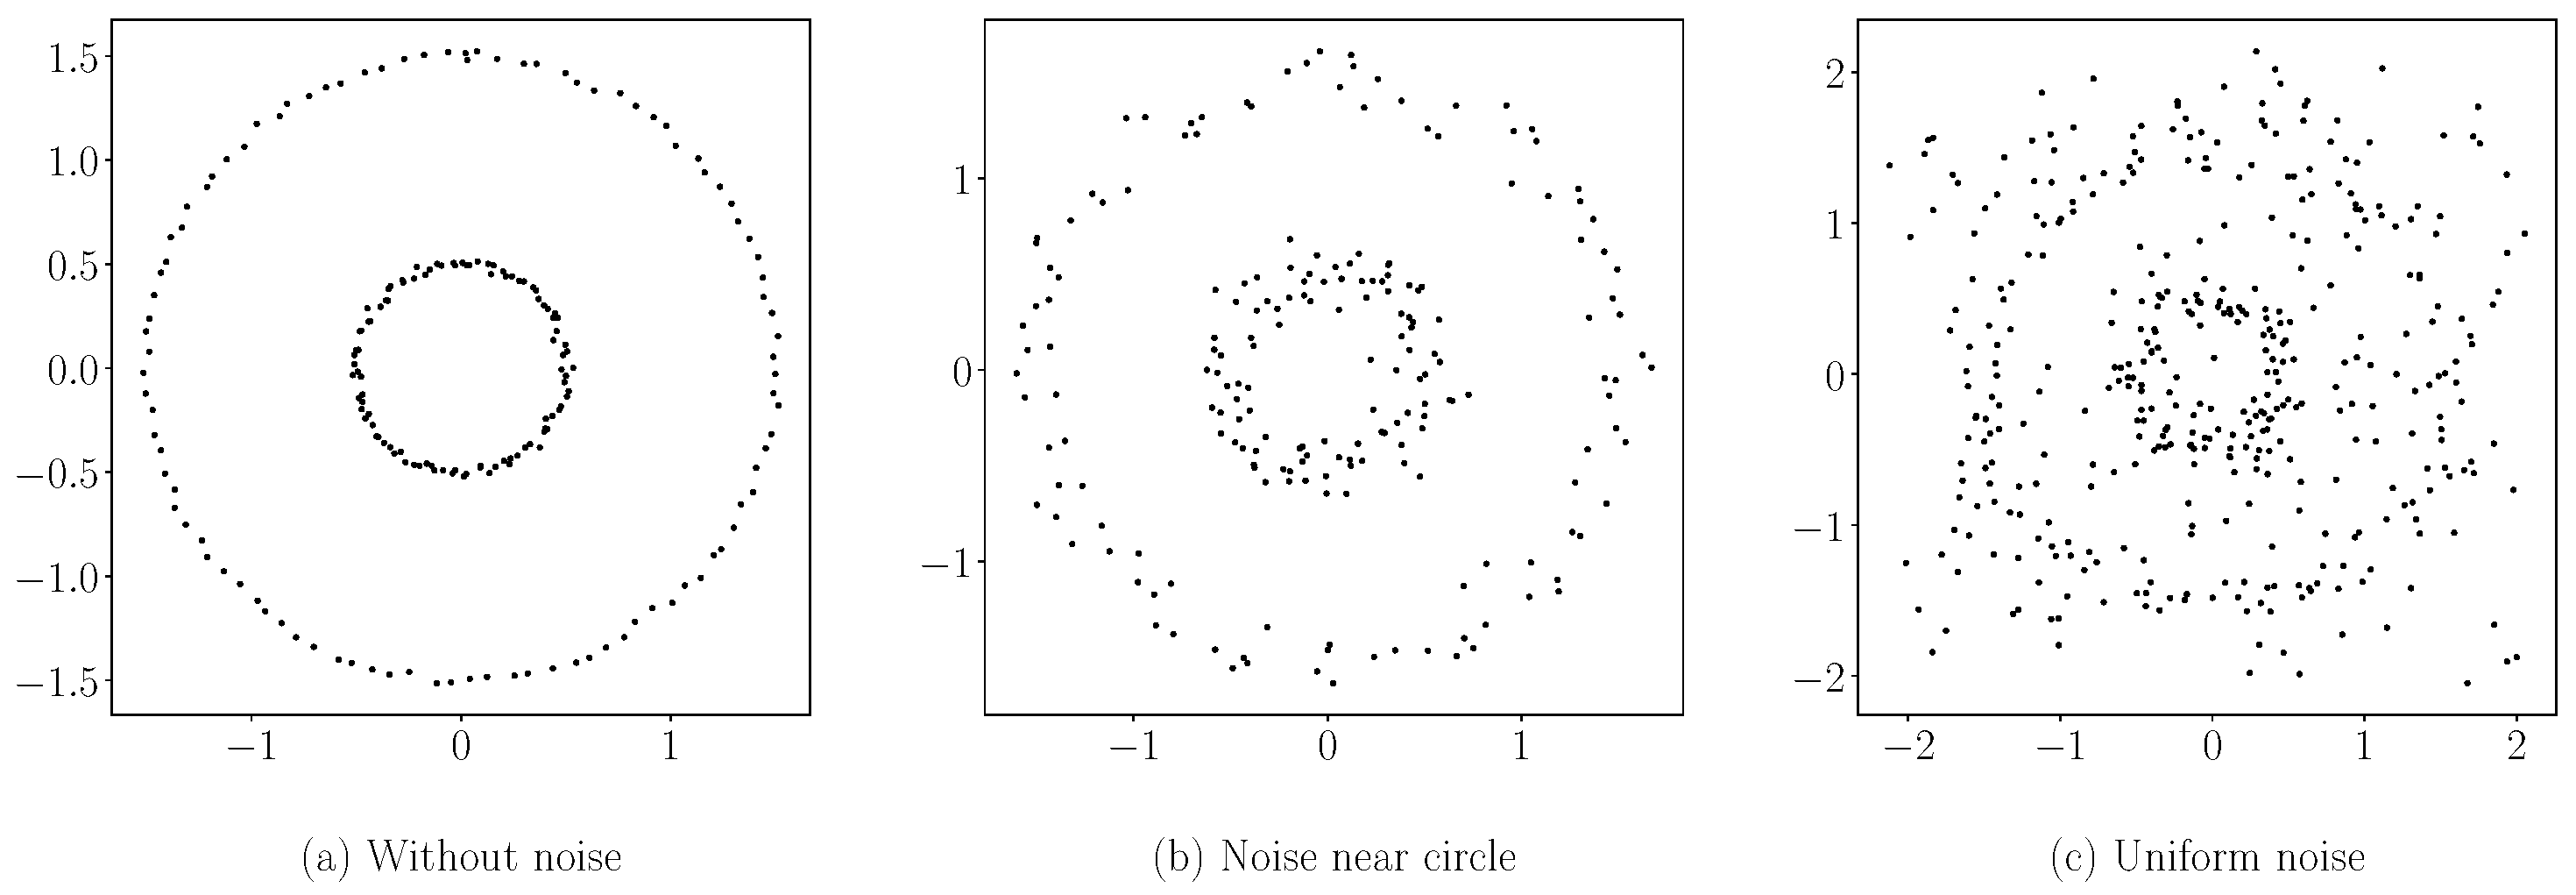
\includegraphics[width=1\textwidth]{result_eng/statment}
\caption{An example of circles with different noise levels: (a) circle without noise; (b) noisy radius circle; (c) noisy radius circle, and uniform noisy on image}
\label{example:1}
\end{figure}

The paper analysis multimodel quality depending on the prior distribution of the expert's parameters.
There solves a problem of finding circles on a binarized image.
Examples of images are shown in fig.~\ref{example:1}.
In this paper, each expert is a linear model.
A gate function is a two-layer fully connected neural network.

\section{Related work}
Many papers on a mixture of experts are devoted to the choice of a gateway function: softmax, the Dirichlet process~\cite{Edward2002}, a neural network~\cite{Shazeer2017} with softmax function on the last layer.
Some papers are devoted to the choice of expert type. 
Papers~\cite{Jordan1994, Jordan1991} analyze linear models as experts.
Papers~\cite{Lima2007, Cao2003} analyze SVMs as experts.
The paper~\cite{Yuksel2012} contains an overview of different methods for choosing a gate function and expert type.

A mixture of experts has many applications.
Papers~\cite{Yumlu2003, Cheung1995, Weigend2000} use a mixture of experts in the task of forecasting time series.
The paper~\cite{Ebrahimpour2009} uses a mixture of experts in the task of recognizing handwritten numbers.
Papers~\cite{Estabrooks2001, Mossavat2010, Peng1996, Tuerk2001}  are devoted to methods of text and speech recognition by using a mixture of experts.
The paper~\cite{Sminchisescu2007} analyzes a mixture of experts in the task of recognizing three-dimensional human movements.

The paper~\cite{Bowyer2010} is devoted to a review of the study results on the iris detection in the image.
The methods of highlighting the borders of the iris and pupil are described in papers~\cite{Matveev2010, Matveev2014}.

\section{Problem statement of circle parameters estimation}
This data are binary image
\[
\label{eq:st:cr:1}
\begin{aligned}
\textbf{M} \in \{0,1\}^{m_1 \times m_2},
\end{aligned}
\]
where~$1$ is a black pixel, an image, and $0$ is a white pixel, the image background.
The image~$\textbf{M}$ is mapped to a set of coordinates~$\textbf{C}=\left\{x_i, y_i\right\}_{i=1}^{N}$. The pair of coordinates~$(x_i, y_i)$ is a black pixel in~$\textbf{M}$:
\[
\label{eq:st:cr:2}
\begin{aligned}
\textbf{C} \in  \mathbb{R}^{N \times 2},
\end{aligned}
\]
%где $N$ --- число черных точек на изображении $\textbf{M}$.
where~$N$ is the number of black pixels.

%Обозначим $x_0, y_0$ --- центр окружности, которую требуется найти на бинарном изображении $\textbf{M}$, а $r$ ее радиус.
Let~$(x_0, y_0)$ be the center of the circle, and $r$ is radius of the circle.
%The circle parameters $x_0, y_0, r$ need to be found.
 
%Элементы выборки $\left(x_i, y_i\right)\in\textbf{C}$ являются геометрическим местом точек, которое аппроксимируется уравнением окружности:
The coordinates $\left(x_i, y_i\right)\in\textbf{C}$ is a circle locus of points defined by
\[
\label{eq:st:cr:3}
\begin{aligned}
\left(x_i - x_0\right)^{2}+\left(y_i-y_0\right)^2 = r^2.
\end{aligned}
\]
%Раскрыв скобки получим уравнение
Expand brackets:
\[
\label{eq:st:cr:4}
\begin{aligned}
(2x_0)\cdot x_i + (2y_0)\cdot y_i+(r^2-x_0^2-y_0^2)\cdot1 = x_{i}^2 + y_{i}^2.
\end{aligned}
\]
%Поставим задачу линейной регрессии для нахождения окружности:
Rewrite equation~\eqref{eq:st:cr:4} to set the linear regressions problem for all points in the dataset:
\[
\label{eq:st:cr:5}
\begin{aligned}
\textbf{X}\textbf{w} \approx \textbf{y},  \quad \textbf{X} = \left[\textbf{C}, \textbf{1}\right], \quad \textbf{y} = [x_1^2+y_1^2, x_2^2+y_2^2, \cdots, x_N^2+y_N^2]^{\mathsf{T}}.
\end{aligned}
\]
%где найденые оптимальные параметры линейной регрессии $\textbf{w} = \bigr[w_1, w_2, w_3\bigr]^{\mathsf{T}}$ восстанавливают параметры окружности:
The parameters~$\textbf{w} = \bigr[w_1, w_2, w_3\bigr]^{\mathsf{T}}$ reconstruct the circle parameters~$x_0, y_0, r$:
\[
\label{eq:st:cr:6}
\begin{aligned}
x_0 = \frac{w_1}{2}, \quad y_0 = \frac{w_2}{2}, \quad r = \sqrt[]{w_3+x_{0}^{2}+y_{0}^{2}}.
\end{aligned}
\]

%Решение уравнения~\eqref{eq:st:cr:5} находит параметры единственной окружности на изображении.
The solution of problem~\eqref{eq:st:cr:5} reconstructs the circle parameters only if the number of circles in an image is equal to one.
%В случае, когда на изображении несколько окружностей, предлагается использовать мультимодель.
The authors propose to use the multimodel for the image, which consists of several circles.
%В ее состав входят линейные модели.
The multimodel is an ensemble of the linear models.
%Каждая линейная модель описывает одну окружность на изображении. 
Each linear model approximates only one circle in the image.
%В качестве мультимодели рассматривается смесь экспертов. 
In this paper, multimodel is a mixture of experts.
%Данная постановка обобщается на поиск параметров эллипсов в приложении~\eqref{apendix:el}.

\section{Problem statement of building a mixture of experts}
\begin{definition}
\label{def:1}
%Смесь экспертов~---~мультимодель, определяющая правдоподобие веса $\pi_k$ каждой локальной модели $\textbf{f}_k$ на признаковом описании объекта $\textbf{x}$.
A model~$\mathbf{f}$ is a local model on dataset~$\textbf{X}$ if~model $\mathbf{f}$ approximate some not empty subset~$\textbf{X}'\subset\textbf{X}$.
\end{definition}
Generalize one-circle approximation problem to the case of several circles.
Each circle is a local model.
%Задана выборка из уравнения~\eqref{eq:st:cr:5} :
%The data from equation~\eqref{eq:st:cr:5} for several circles case, given by the following data:
The data for this case is
\[
\label{eq:st:1}
\begin{aligned}
\textbf{X} \in \mathbb{R}^{N \times n},
\end{aligned}
\]
%где~$N$~---~число объектов в выборке, а~$n$~---~размерность признакового пространства.
where~$N$ is a number of datum and~$n$ is a number of features. In this paper,~$n$ is equal to 3.



\begin{definition}
\label{def:2}
%Смесь экспертов~---~мультимодель, определяющая правдоподобие веса $\pi_k$ каждой локальной модели $\textbf{f}_k$ на признаковом описании объекта $\textbf{x}$.
Call the multimodel~$\hat{\mathbf{f}}$ a mixture of experts if
\[
\label{eq:st:2}
\begin{aligned}
\hat{\mathbf{f}} = \sum_{k=1}^{K}\pi_{k}\mathbf{f}_k, \qquad \pi_{k}\left(\mathbf{x}, \mathbf{V}\right):\mathbb{R}^{n\times \left|\mathbf{V}\right|} \to [0, 1], \qquad \sum_{k=1}^{K}\pi_{k}\left(\mathbf{x}, \mathbf{V}\right) = 1,
\end{aligned}
\]
%где~$\hat{\mathbf{f}}$~---~мультимодель, а $\mathbf{f}_k$ является некоторой моделью, $\pi_k$~---~шлюзовая функция, $\mathbf{w}_k$~---~параметры $k$-й локальной модели, $\mathbf{V}$~---~параметры шлюзовой функции.
where~$\mathbf{f}_k$ is a local model, $\pi_k$ is a gate function, vector~$\mathbf{w}_k$ is some parameters of the local model and~$\mathbf{V}$ is some parameters of the gate function.
\end{definition}



%В данной работе в качестве локальных моделей~$\mathbf{f}_k$ и шлюзовой функции~$\bm{\pi}$ рассматриваются следующие функции:
This paper asserts the local model a linear model. The gate function is the two--layer fully connected neural network
\[
\label{eq:st:3}
\begin{aligned}
\mathbf{f}_k\left(\textbf{x}\right) = \textbf{w}_k^{\mathsf{T}}\textbf{x}, \quad
\bm{\pi}\left(\mathbf{x}, \mathbf{V}\right) = \text{softmax}\bigr(\mathbf{V}_{1}^{\mathsf{T}}\bm{\sigma}\left(\mathbf{V}_2^{\mathsf{T}}\mathbf{x}\right)\bigr),
\end{aligned}
\]
%где $\mathbf{V} = \bigr\{\mathbf{V}_1, \mathbf{V}_2\bigr\}$~---~параметры шлюзовой функции.
where $\mathbf{V} = \bigr\{\mathbf{V}_1, \mathbf{V}_2\bigr\}$ is a set of the gate function parameters.

%Параметры локальных моделей оптимизируются согласно принципу максимального правдоподобия модели:
%All parameters optimises according to the maximum likelihood principle:
%Recall from~\eqref{eq:st:2} that the full distribution can be written as a linear superposition of local distribution:
Combining~\eqref{eq:st:2} and~\eqref{eq:st:3}, obtain the likelihood solution:
\[
\label{eq:st:4}
\begin{aligned}
p\bigr(\mathbf{y}, \mathbf{W}|\mathbf{X}, \mathbf{V}\bigr) = \prod_{k=1}^{K}p^{k}\bigr(\mathbf{w}_k\bigr)\prod_{i=1}^{N}\left(\sum_{k=1}^{K}\pi_{k}p_{k}\bigr(y_i|\mathbf{w}_k, \mathbf{x}_i\bigr)\right),
\end{aligned}
\]
%где $\mathbf{W} = \bigr[\mathbf{w}_1, \mathbf{w}_2, \cdots, \mathbf{w}_K\bigr]^{\mathsf{T}}.$
where~$\mathbf{W} = \bigr[\mathbf{w}_1, \mathbf{w}_2, \cdots, \mathbf{w}_K\bigr]^{\mathsf{T}}.$

%Задача оптимизации параметров локальных моделей и параметров смеси:
%The optimisation problem for finding optimal parameters of local models and optimal mixture parameters:
The optimal parameters is delivered by the maximum likelihood solution:
\[
\label{eq:st:5}
\begin{aligned}
\hat{\mathbf{W}}, \hat{\mathbf{V}} = \arg\max_{\mathbf{W}, \mathbf{V}} p\bigr(\mathbf{y}, \mathbf{W}|\mathbf{X}, \mathbf{V}\bigr).
\end{aligned}
\]

\section{EM--algorithm as a solver of optimisation problem }
%Для построения смеси экспертов рассмотрим следующую вероятностную постановку задачи. Предположим, что
To build a mixture of experts, set the following probabilistic statement for the problem~\eqref{eq:st:1}:

\begin{enumerate}
	%\item[1)] правдоподобие выборки $p_{k}\left(y_{i}|\mathbf{w}_{k}, \mathbf{x}_{i}\right) = \mathcal{N}\left(y_{i}|\mathbf{w}_{k}^{\mathsf{T}}\mathbf{x}_{i}, \beta^{-1}\right),$ где $\beta$ уровень шума,
	\item[1)] a likelihood $p_{k}\left(y_{i}|\mathbf{w}_{k}, \mathbf{x}_{i}\right) = \mathcal{N}\left(y_{i}|\mathbf{w}_{k}^{\mathsf{T}}\mathbf{x}_{i}, \beta^{-1}\right).$ Parameter~$\beta$ is a level of noise,
	%\item[2)] априорное распределение параметров $p^{k}\left(\mathbf{w}_{k}\right) = \mathcal{N}\left(\mathbf{w}_{k}|\mathbf{w}^{0}_{k}, \mathbf{A}_{k}\right),$ где $\mathbf{w}^{0}_{k}$~---~вектор размера $n\times1,$ $\mathbf{A}_{k}$~---~ковариационная матрица параметров,
	\item[2)] a prior distribution of parameters $p^{k}\left(\mathbf{w}_{k}\right) = \mathcal{N}\left(\mathbf{w}_{k}|\mathbf{w}^{0}_{k}, \mathbf{A}_{k}\right),$ where $\mathbf{w}^{0}_{k}$ is a vector of size $n\times1$ and~$\mathbf{A}_{k}$ is a covariance matrix,
	%\item[3)] регуляризация априорного распределения $p\left(\bm{\varepsilon}_{k,k'}|\bm{\alpha}\right) = \mathcal{N}\left(\bm{\varepsilon}_{k,k'}|\mathbf{0},  \bm{\Xi}\right),$ где~$\bm{\Xi}$~---~ковариационная матрица общего вида, $\bm{\varepsilon}_{k,k'} = \mathbf{w}_{k}^{0}-\mathbf{w}_{k'}^{0}.$
	\item[3)] prior regularisation $p\left(\bm{\varepsilon}_{k,k'}|\bm{\Xi}\right) = \mathcal{N}\left(\bm{\varepsilon}_{k,k'}|\mathbf{0},  \bm{\Xi}\right),$ where~$\bm{\Xi}$ is a covariance matrix and $\bm{\varepsilon}_{k,k'} = \mathbf{w}_{k}^{0}-\mathbf{w}_{k'}^{0}.$
\end{enumerate}
%Тогда правдоподобие модели~\eqref{eq:st:4} переписывается в следующем виде:
%The previous assumption, the likelihood~\eqref{eq:st:4} is rewritten to:
%The previous assumption allows us to rewrite the likelihood from equation~\eqref{eq:st:4}:
Combining assumptions~$1), 2), 3)$ and equation~\eqref{eq:st:4}, obtain
\[
\label{eq:em:1}
\begin{aligned}
p\bigr(\mathbf{y}, \mathbf{W}|\mathbf{X}, \mathbf{V}, \textbf{A}, \textbf{W}^{0}, \bm{\Xi}, \beta\bigr) = &\prod_{k,k'=1}^{K}\mathcal{N}\left(\bm{\varepsilon}_{k,k'}|\mathbf{0},  \bm{\Xi}\right)\cdot\\
&\cdot\prod_{k=1}^{K}\mathcal{N}\left(\mathbf{w}_{k}|\mathbf{w}^{0}_{k}, \mathbf{A}_{k}\right)\prod_{i=1}^{N}\left(\sum_{k=1}^{K}\pi_{k}\mathcal{N}\left(y_{i}|\mathbf{w}_{k}^{\mathsf{T}}\mathbf{x}_{i}, \beta^{-1}\right)\right),
\end{aligned}
\]
%где~$\mathbf{A} = \bigr\{\mathbf{A}_1, \cdots, \mathbf{A}_K\bigr\}.$
 where~$\mathbf{A} = \bigr\{\mathbf{A}_1, \cdots, \mathbf{A}_K\bigr\}.$
 
%Для решения задачи~\eqref{eq:st:5} в предположении~\eqref{eq:em:1} введем матрицу скрытых переменных~$\mathbf{Z}$, где $z_{ik} = 1$, если $i$-й~объект порожден моделью~$k$ и~$z_{ik} = 0$ иначе.
%Consider the matrix of hidden variables~$\mathbf{Z}$ for solving problem~\eqref{eq:st:5} under assumption~\eqref{eq:em:1}. In matrix~$\mathbf{Z}$ all~$z_{ik} = 1$ if and only if object $i$ related to local model $k$ and $z_{ik} = 0$ otherwise.
Introduce a binary matrix~$\mathbf{Z}$. Its element~$z_{ik}$ is equal to $1$ if and only if the object $i$ is related to the local model $k$.
%If we combine the binary matrix~$\mathbf{Z}$ with logarithm of likelihood~\eqref{eq:em:1}, we get
Integrating the binary matrix~$\mathbf{Z}$ in~\eqref{eq:em:1}, obtain:
\[
\label{eq:em:2}
\begin{aligned}
\log p\bigr(\mathbf{y}, \mathbf{Z}, \mathbf{W}&|\mathbf{X}, \mathbf{V}, \textbf{A}, \textbf{W}^{0},  \bm{\Xi}, \beta\bigr) =\\
&= \sum_{i=1}^{N}\sum_{k=1}^{K}z_{ik}\left[\log\pi_k\left(\textbf{x}_i, \textbf{V}\right) - \frac{\beta}{2}\left(y_{i} - \textbf{w}_{k}^{\mathsf{T}}\textbf{x}_{i}\right)^{2} + \frac{1}{2}\log\frac{\beta}{2\pi}\right] +\\
&+ \sum_{k=1}^{K}\left[-\frac{1}{2}\left(\textbf{w}_{k} - \textbf{w}_{k}^{0}\right)^{\mathsf{T}}\textbf{A}_{k}^{-1}\left(\textbf{w}_{k} - \textbf{w}_{k}^{0}\right) + \frac{1}{2}\log\det\textbf{A}^{-1}_{k} - \frac{n}{2}\log2\pi\right]+\\
&+ \sum_{k=1}^{K}\sum_{k'=1}^{K}\left[-\frac{1}{2}\left(\textbf{w}_{k}^{0}-\textbf{w}_{k'}^{0}\right)^{\mathsf{T}}\bm{\Xi}^{-1}\left(\textbf{w}_{k}^{0}-\textbf{w}_{k'}^{0}\right) +\frac{1}{2}\log\det \bm{\Xi} -\frac{n}{2}\log{2\pi}\right].
\end{aligned}
\]
%С учетом~\eqref{eq:em:2} задача оптимизации~\eqref{eq:st:5} принимает вид:
%The optimisation problem~\eqref{eq:st:5} for log--likelihood~\eqref{eq:em:2} rewrites as follows
Obtain a new optimisation problem combining~\eqref{eq:st:5} and~\eqref{eq:em:2}:
\[
\label{eq:em:3}
\begin{aligned}
\mathbf{W}, \mathbf{Z}, \mathbf{V}, \mathbf{W}^0, \textbf{A},  \beta = \arg\max_{\mathbf{W}, \mathbf{Z}, \mathbf{V}, \mathbf{W}^0, \textbf{A}, \beta} \log p\bigr(\mathbf{y}, \mathbf{Z}, \mathbf{W}&|\mathbf{X}, \mathbf{V}, \textbf{A}, \textbf{W}^{0}, \bm{\Xi}, \beta\bigr).
\end{aligned}
\]
%Для поиска локального минимума в задаче оптимизации~\eqref{eq:em:3} воспользуемся вариационным EM--алгоритмом.
Use the expectation-maximization~\cite{bishop2006} algorithm to find the maximum likelihood solution~\eqref{eq:em:3} for the multimodel~\eqref{eq:em:1} with latent variable~$\mathbf{Z}$.

\paragraph{E--step.} 
%Найдем вариационной распределение~\cite{bishop2006} в условиях аппроксимации среднего поля $q\left(\mathbf{Z}, \mathbf{W}\right) = q\left(\mathbf{Z}\right)q\left(\mathbf{W}\right)$ наиболее близкое к $p\bigr(\mathbf{Z}, \mathbf{W}|\mathbf{y}, \mathbf{X}, \mathbf{V}, \textbf{A}, \textbf{W}^{0}, \bm{\Xi}, \beta\bigr)$.
Let a join distribution~$q\left(\mathbf{Z}, \mathbf{W}\right)$ satisfies  the following assumption~$q\left(\mathbf{Z}, \mathbf{W}\right) = q\left(\mathbf{Z}\right)q\left(\mathbf{W}\right)$~\cite{bishop2006}. 
%Find the variational distribution~$q\left(\mathbf{Z}, \mathbf{W}\right)$ closest to~$p\bigr(\mathbf{Z}, \mathbf{W}|\mathbf{y}, \mathbf{X}, \mathbf{V}, \textbf{A}, \textbf{W}^{0}, \bm{\Xi}, \beta\bigr)$.
%Для упрощения будем искать логарифм с точностью до аддитивной константы, которую восстановим используя вид распределения.
The symbol~$\propto$ means that both sides are equal to up to an additive constant.
%Найдем распределение скрытой переменной~$q\left(\textbf{Z}\right)$
First, find the distribution~$q\left(\textbf{Z}\right)$:
\[
\label{eq:em:4}
\begin{aligned}
\log q\left(\textbf{Z}\right) &= \mathsf{E}_{q/\textbf{Z}} \log p\bigr(\mathbf{y}, \mathbf{Z}, \mathbf{W}|\mathbf{X}, \mathbf{V}, \textbf{A}, \textbf{W}^{0}, \bm{\Xi}, \beta\bigr)  \propto\\
&\propto \sum_{i+1}^{N}\sum_{k=1}^{K}z_{ik}\left[\log\pi_{k}\left(\textbf{x}_{i}, \textbf{V}\right) - \frac{\beta}{2}\left(y_{i}^{2} -\textbf{x}_{i}^{\mathsf{T}}\mathsf{E}\textbf{w}_{k} + \textbf{x}_{i}^{\mathsf{T}}\mathsf{E}\textbf{w}_{k}\textbf{w}_{k}^{\mathsf{T}}\textbf{x}_{i}\right) + \frac{1}{2}\log\frac{\beta}{2\pi}\right]\\
p\left(z_{ik} = 1\right) &= \frac{\exp\left(\log\pi_{k}\left(\textbf{x}_{i}, \textbf{V}\right) - \frac{\beta}{2}\left(\textbf{x}_{i}^{\mathsf{T}}\mathsf{E}\textbf{w}_{k}\textbf{w}_{k}^{\mathsf{T}}\textbf{x}_{i} - \textbf{x}_{i}^{\mathsf{T}}\mathsf{E}\textbf{w}_{k}\right)\right)}{\sum_{k'=1}^{K}\exp\left(\log\pi_{k'}\left(\textbf{x}_{i}, \textbf{V}\right) - \frac{\beta}{2}\left(\textbf{x}_{i}^{\mathsf{T}}\mathsf{E}\textbf{w}_{k'}\textbf{w}_{k'}^{\mathsf{T}}\textbf{x}_{i} - \textbf{x}_{i}^{\mathsf{T}}\mathsf{E}\textbf{w}_{k'}\right) \right)}.
\end{aligned}
\]
%Получаем, что распределениие $q\bigr(z_{ik}\bigr)$ является бернулевским с параметром~$z_{ik}$ из выражения~\eqref{eq:em:4}.
The distribution~$q\bigr(z_{ik}\bigr)$ is the Bernoulli distribution with probability~$z_{ik}$ from equation~\eqref{eq:em:4}.
%Найдем распределение переменной~$q\left(\textbf{W}\right)$
Second, find the distribution~$q\left(\textbf{W}\right)$:
\[
\label{eq:em:5}
\begin{aligned}
\log q\left(\textbf{W}\right) &= \mathsf{E}_{q/\textbf{W}}\log p\bigr(\mathbf{y}, \mathbf{Z}, \mathbf{W}|\mathbf{X}, \mathbf{V}, \textbf{A}, \textbf{W}^{0}, \bm{\Xi}, \beta\bigr) \propto\\
&\propto \sum_{i=1}^{N}\sum_{k=1}^{K}\mathsf{E}z_{ik}\left[\log\pi_{k}\left(\textbf{x}_{i, \textbf{V}}\right) - \frac{\beta}{2}\left(y_{i} - \textbf{w}_{k}^{\mathsf{T}}\textbf{x}_{i}\right)^{2} + \frac{1}{2}\log\frac{\beta}{2\pi}\right] + \\
&+ \sum_{k=1}^{K}\left[-\frac{1}{2}\left(\textbf{w}_{k} - \textbf{w}_{k}^{0}\right)^{\mathsf{T}}\textbf{A}_{k}^{-1}\left(\textbf{w}_{k} - \textbf{w}_{k}^{0}\right) + \frac{1}{2}\log\det\textbf{A}^{-1}_{k} - \frac{n}{2}\log2\pi\right] \\
&\propto \sum_{k=1}^{K}\left[\textbf{w}_{k}^{\mathsf{T}}\left(\textbf{A}_{k}^{-1}\textbf{w}_{k}^{0}+\beta\sum_{i=1}^{N}\textbf{x}_{i}y_{i}\mathsf{E}z_{ik}\right)-\frac{1}{2}\textbf{w}_{k}^{\mathsf{T}}\left(\textbf{A}_{k}^{-1}+\beta\sum_{i=1}^{N}\textbf{x}_{i}\textbf{x}_{i}^{\mathsf{T}}\right)\textbf{w}_{k}\right].
\end{aligned}
\]
%Из вида распределения~\eqref{eq:em:5} получаем, что распределение $q\bigr(\mathbf{w}_{k}\bigr) = \mathcal{N}\left(\mathbf{w}_{k}| \mathbf{m}_{k}, \mathbf{B}_k\right),$ является нормальным с параметрами $\mathbf{m}_k, \mathbf{B}_k,$ которые определяются следующим образом:
The distribution~$q\bigr(\mathbf{w}_{k}\bigr)$ is the normal distribution with mean~$\mathbf{m}_{k}$ and covariance matrix~$\mathbf{B}_k$:
\[
\label{eq:em:6}
\begin{aligned}
\mathbf{m}_{k} = \mathbf{B}_{k}\left(\mathbf{A}_{k}^{-1}\mathbf{w}_{k}^{0}+\beta\sum_{i=1}^{N}\mathbf{x}_{i}y_{i}\mathsf{E}z_{ik}\right), \qquad \mathbf{B}_{k} = \left(\mathbf{A}_{k}^{-1}+\beta\sum_{i=1}^{N}\mathbf{x}_{i}\mathbf{x}_{i}^{\mathsf{T}}\mathsf{E}z_{ik}\right)^{-1}.
\end{aligned}
\]

\paragraph{M--step.} 
%Найдем $\mathbf{V}, \mathbf{W}^0, \textbf{A},  \beta$ из максимизации~$\mathsf{E}_{q}\log p\bigr(\mathbf{y}, \mathbf{Z}, \mathbf{W}|\mathbf{X}, \mathbf{V}, \textbf{A}, \textbf{W}^{0}, \bm{\Xi}, \beta\bigr)$.
The distribution~$q\left(\mathbf{Z}, \mathbf{W}\right)$ is fixed, while the lower bound~$\mathcal{L}\left(\textbf{V}, \textbf{W}^{0}, \textbf{A}, \beta\right)$  is maximized with respect to the parameters~$\mathbf{V}, \mathbf{W}^0, \textbf{A},  \beta$:
\[
\label{eq:em:7}
\begin{aligned}
\mathcal{L}\left(\textbf{V}, \textbf{W}^{0}, \textbf{A}, \beta\right) &= \mathsf{E}_{q}\log p\bigr(\mathbf{y}, \mathbf{Z}, \mathbf{W}|\mathbf{X}, \mathbf{V}, \textbf{A}, \textbf{W}^{0}, \bm{\Xi}, \beta\bigr) =  \\
&= \sum_{i=1}^{N}\sum_{k=1}^{K}\mathsf{E}z_{ik}\left[\log\pi_k\left(\textbf{x}_i, \textbf{V}\right) - \frac{\beta}{2}\mathsf{E}\left(y_{i} - \textbf{w}_{k}^{\mathsf{T}}\textbf{x}_{i}\right)^{2} + \frac{1}{2}\log\frac{\beta}{2\pi}\right] +\\
&+ \sum_{k=1}^{K}\left[-\frac{1}{2}\mathsf{E}\left(\textbf{w}_{k} - \textbf{w}_{k}^{0}\right)^{\mathsf{T}}\textbf{A}_{k}^{-1}\left(\textbf{w}_{k} - \textbf{w}_{k}^{0}\right) + \frac{1}{2}\log\det\textbf{A}^{-1}_{k} - \frac{n}{2}\log2\pi\right] +\\
&+ \sum_{k=1}^{K}\sum_{k'=1}^{K}\left[-\frac{1}{2}\left(\textbf{w}_{k}^{0}-\textbf{w}_{k'}^{0}\right)^{\mathsf{T}}\bm{\Xi}^{-1}\left(\textbf{w}_{k}^{0}-\textbf{w}_{k'}^{0}\right) +\frac{1}{2}\log\det\bm{\Xi} -\frac{n}{2}\log{2\pi}\right].
\end{aligned}
\]
%Для нахождения параметров~$\textbf{V}$ максимизирующих функцию~\eqref{eq:em:7} воспользуемся градиентным методом оптимизации. 
To find the optimal parameters~$\textbf{V}$, use the gradient optimization algorithm.
%Он гарантирует сходимость к локальному экстремуму функции.
It convergences to some local maximum.
%Оптимальное значение параметра~$\textbf{A}_k$, которое максимизирует функцию~\eqref{eq:em:7}, найдем из условия оптимума первого порядка:
%Let find the parameters~$\textbf{A}_k$, which maximising the function~\eqref{eq:em:7}:
Using~\eqref{eq:em:7}, we get
\[
\label{eq:em:9}
\begin{aligned}
\frac{\partial \mathcal{L}\left(\textbf{V}, \textbf{W}^{0}, \textbf{A}, \beta\right)}{\partial \textbf{A}^{-1}_k} &=  \frac{1}{2}\textbf{A}_{k} - \frac{1}{2}\mathsf{E}\left(\textbf{w}_{k} - \textbf{w}_{k}^{0}\right)\left(\textbf{w}_{k} - \textbf{w}_{k}^{0}\right)^{\mathsf{T}} = 0,\\
\textbf{A}_{k} &= \mathsf{E}\textbf{w}_{k}\textbf{w}_{k}^{\mathsf{T}} - \textbf{w}_{k}^{0}\mathsf{E}\textbf{w}_{k}^{\mathsf{T}} - \mathsf{E}\textbf{w}_{k}\textbf{w}_{k}^{0\mathsf{T}} + \textbf{w}_{k}^{0}\textbf{w}_{k}^{0\mathsf{T}}.
\end{aligned}
\]
%Аналогично найдем оптимальные значения~$\beta$ и~$\textbf{w}_0^{k}$.
Similarly, we get
\[
\label{eq:em:10}
\begin{aligned}
\frac{\partial \mathcal{L}\left(\textbf{V}, \textbf{W}^{0}, \textbf{A}, \beta\right)}{\partial \beta} &= \sum_{k=1}^{K}\sum_{i=1}^{N}\left(\frac{1}{\beta}\mathsf{E}z_{ik}-\frac{1}{2}\mathsf{E}z_{ik}\left[y_{i}^{2}-2y_{i}\textbf{x}_{i}^{\mathsf{T}}\mathsf{E}\textbf{w}_{k}+\textbf{x}_{i}^{\mathsf{T}}\textbf{w}_{k}\textbf{w}_{k}^{\mathsf{T}}\textbf{x}_{i}\right]\right) = 0,\\
\frac{1}{\beta}&=\frac{1}{N}\sum_{i=1}^{N}\sum_{k=1}^{K}\left[y_{i}^{2}-2y_{i}\textbf{x}_{i}^{\mathsf{T}}\mathsf{E}\textbf{w}_{k} + \textbf{x}_{i}^{\mathsf{T}}\mathsf{E}\textbf{w}_{k}\textbf{w}_{k}^{\mathsf{T}}\textbf{x}_{i}\right]\mathsf{E}z_{ik}.
\end{aligned}
\]
\[
\label{eq:em:11}
\begin{aligned}
\frac{\partial \mathcal{L}\left(\textbf{V}, \textbf{W}^{0}, \textbf{A}, \beta\right)}{\partial \mathbf{w}_k^0} &= \mathbf{A}_k^{-1}\bigr(\mathsf{E}\mathbf{w}_k - \mathbf{w}_{k}^{0}\bigr) + \bm{\Xi}\sum_{k'=1}^{K}\bigr[\mathbf{w}_{k'}^{0} -\mathbf{w}_{k}^{0}\bigr] = 0,\\
\textbf{w}_{k}^{0} &=\left[\textbf{A}_{k}^{-1}+\left(K-1\right)\bm{\Xi}\right]^{-1}\left(\textbf{A}^{-1}_{k}\mathsf{E}\textbf{w}_{k}+\bm{\Xi}\sum_{k'=1,~k'\not=k}^{K}\textbf{w}_{k'}^{0}\right).
\end{aligned}
\]
%Используя формулы~(\ref{eq:em:4}--\ref{eq:em:11}) получаем итеративную процедуру, которая сходится к локальному максимуму~\eqref{eq:em:3}.
Formulas~(\ref{eq:em:4}--\ref{eq:em:11}) define an iterative procedure, which convergence to some local maximum of the optimization problem~\eqref{eq:em:3}.

%Если в списке вероятностных предположений оставить только пункт~1) получим решение задачи оптимизации~\eqref{eq:em:1}, когда не задано никаких априорных распределений на модели. 
%If in the list of probabilistic statements we leave only the statement~1) then we find a solution to the optimization problem~\eqref{eq:em:1}.
%В случае, когда рассматриваются пункты~1),\,2) получим задачу с заданными априорными распределениями параметров локальных моделей.  
%If in the list of probabilistic statements we leave statements~1) and~2) then we find a solution to the optimization problem with prior distribution on each local model parameters.
%В случае, когда рассматриваются все пункты~1),\,2),\,3) назовем решение с регуляризацией априорных распределений, так как в данном случае мы учитываем зависимость между локальными моделями.
%If in the list of probabilistic statements we leave all statements~1),~2) and 3) then we find a solution to the optimization problem~\eqref{eq:em:3} with prior distributions and relationships between prior distributions of different local models.

\section{Computational experiment}
\begin{comment}
Проводится вычислительный эксперимент для анализа качества моделей нахождения окружностей. В эксперименте рассматривается мультимодель без задания априорных распределений на параметры модели, которую обозначим~$\mathfrak{M}_1$, мультимодель~$\mathfrak{M}_2$ с заданным априорным распределением~\eqref{eq:ce:1} на параметры локальных моделей, также рассматривается мультимодель~$\mathfrak{M}_3$ с регуляризацией априорных распределений.
Качество прогноза моделью~$\mathfrak{M}_i$ окружности определяется функцией
\[
\label{eq:ce:ex:0:1}
\begin{aligned}
\mathcal{S}_{\mathfrak{M}_i} = \sum_{k=1}^{K}\bigr(x^{k}_{0}-x^{k}_{\text{pr}}\bigr)^2+\bigr(y^{k}_{0}-y^{k}_{\text{pr}}\bigr)^2+\bigr(r^{k}-r^{k}_{\text{pr}}\bigr)^2,
\end{aligned}
\]
где $x^{k}_0, y^{k}_0, r^{k}$~---~истинные  значения центра и радиуса $k$-й окружности, $x^{k}_{\text{pr}}, y^{k}_{\text{pr}}, r^{k}_{\text{pr}}$~---~предсказанные значения центра и радиуса $k$-й окружности.

Для сравнения качества моделей с разными априорными распределениями, качество модели оценивается правдоподобием модели без учета априорного распределения:
\[
\label{eq:ce:st:2:1}
\begin{aligned}
\log p\bigr(\mathbf{y}|\mathbf{W}, \mathbf{X}, \mathbf{V}, \beta\bigr) = \sum_{k=1}^{K}\sum_{i=1}^{N}\pi_{k}\bigr(\mathbf{x}_i, \mathbf{V}\bigr)\left[-\frac{\beta}{2}\left(y_i-\mathbf{w}^{\mathsf{T}}\mathbf{x}_i\right)^2-\frac{1}{2}\log{2\pi}+\frac{1}{2}\log\beta\right].
\end{aligned}
\]


Априорные распределения на параметры локальных моделей в эксперименте было задано следующим образом:
\[
\label{eq:ce:1}
\begin{aligned}
p^{1}\left(\textbf{w}_1\right)\sim\mathcal{N}\left(\textbf{w}^{0}_{1}, \textbf{I}\right), \quad p^{2}\left(\textbf{w}_2\right)\sim\mathcal{N}\left(\textbf{w}^{0}_{2}, \textbf{I}\right),
\end{aligned}
\]
где $\textbf{w}^{0}_1 = [0, 0, 0.1],\ \textbf{w}^{0}_2 = [0, 0, 2]$, что указывает на концентричность окружностей и на различность радиусов.

\paragraph{Синтетические данные с разным типом шума в изображении.}
\begin{figure}[h!t]\center
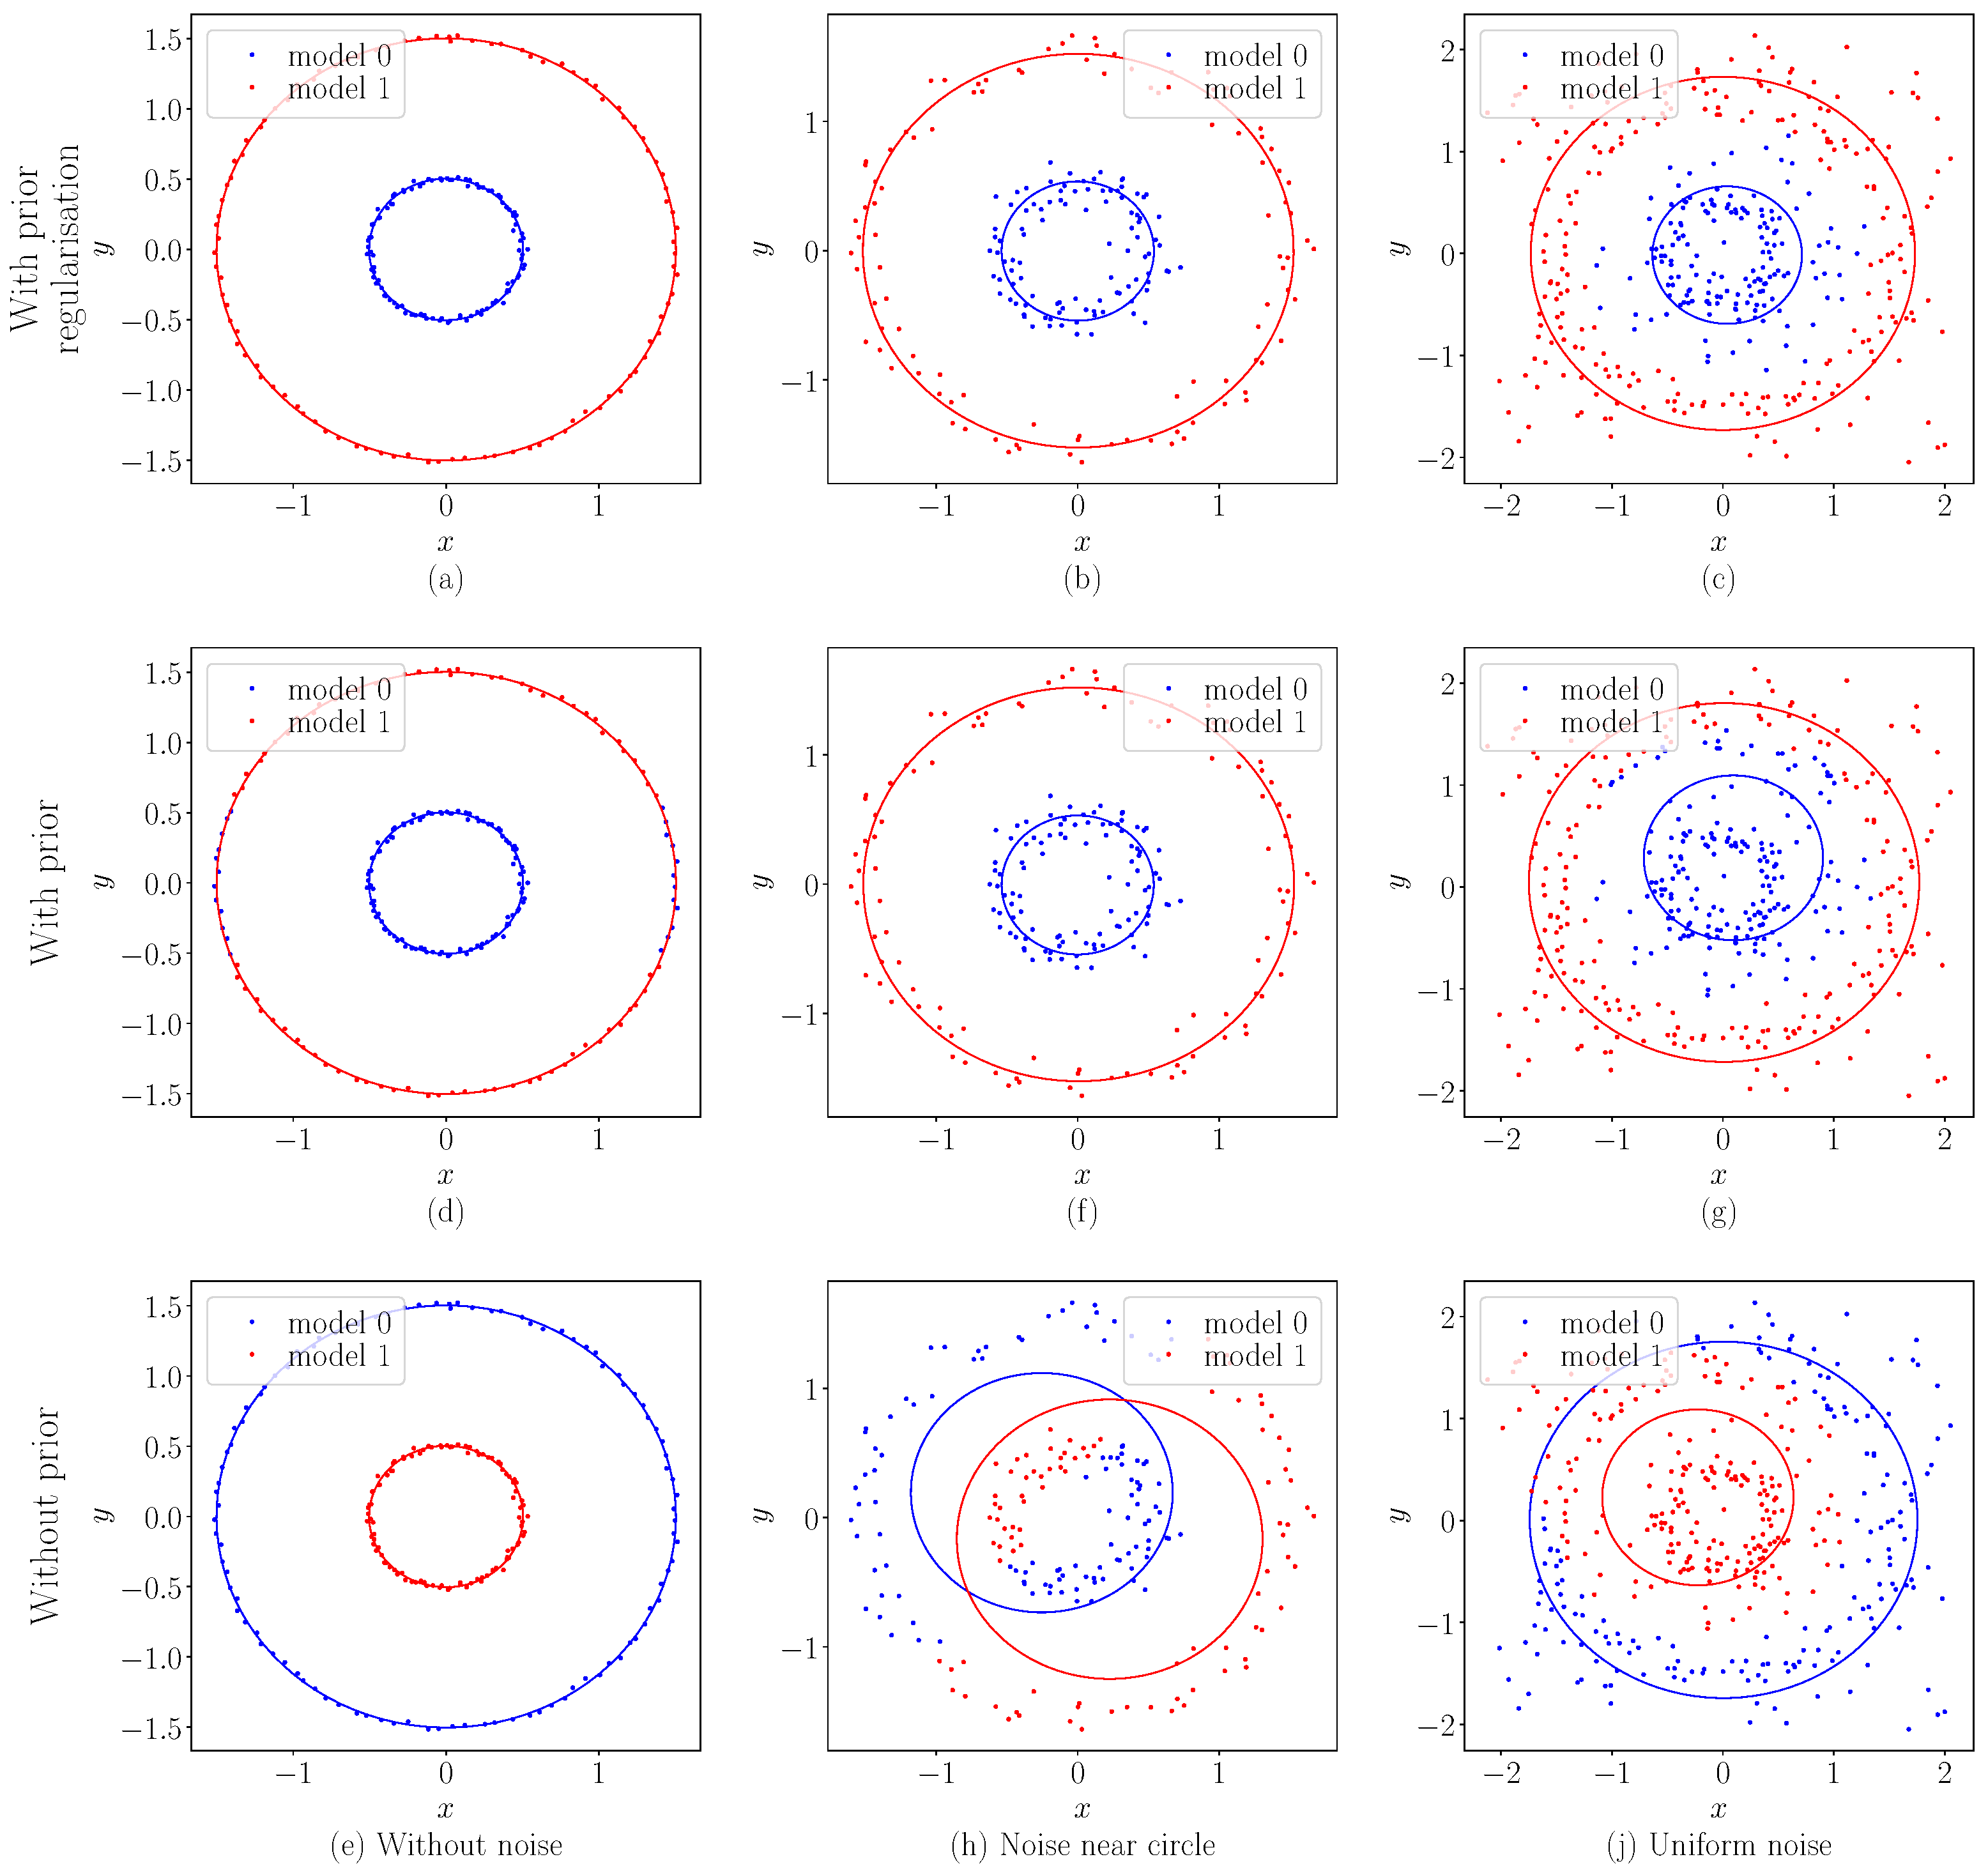
\includegraphics[width=1\textwidth]{result_eng/experiment_synthetic}
\caption{Мультимодель в зависимости от разных априорных предположений и в зависимости от разного уровня шума: (a)--(с) модель с регуляризаций априорных распределений; (d)--(g) модель с заданными априорными распределениями на параметрах локальных моделей; (e)--(j) модель без заданных априорных предположений}
\label{experiment:1}
\end{figure}

Для сравнения качества работы мультимоделей~$\mathfrak{M}_1, \mathfrak{M}_2, \mathfrak{M}_3$ смеси экспертов с разными начальными предположениями был проведен вычислительный эксперимент на синтетических данных. 
%Рассматривалась мультимодель в которойне было задано никаких априорных знаний. Рассматривалась мультимодель, где в качестве априорных знаний задавались априорные распределения на вектора параметров локальных моделей, также рассматривалась мультимодель, где в качестве априорных знаний дополнительно была введена регуляризация априорных распределений.

Вычислительный эксперимент проводится на синтетических выборках, которые получена при помощи генерации двух концентрических окружностей с разным уровнем шума. Выборка Synthetic~1~---~выборка без шума, Synthetic~2~---~выборка с шумом вблизи окружностей, Synthetic~3~---~выборка с шумом вблизи окружности, а также с равномерным шумом по всему изображению.

%Предлагается сравнить две постановки задачи смеси экспертов: в случае когда используются априорные знания об изображении и в случае когда априорные знания отсутствуют. Причем априорные знания задаются двумя разными способами: с регуляризацией априорных распределений и без нее.

На рис.~\ref{experiment:1} показан случайный результаты работы мультимоделей~$\mathfrak{M}_1, \mathfrak{M}_2, \mathfrak{M}_3$. На всех изображениях обе модели обучались $50$ итераций ЕМ--алгоритма. Мультимодели~$\mathfrak{M}_2, \mathfrak{M}_3$ работают лучше мультимодели~$\mathfrak{M}_1$, так как они восстанавливают окружности лучше. Качество прогноза посчитанное по формуле~\eqref{eq:ce:ex:0:1} представлены в табл.~\ref{tb:ce:1}.

\begin{table}[h!t]
\begin{center}
\caption{Результаты работы мультимоделей на синтетических выборках}
\label{tb:ce:1}
\begin{tabular}{|c|c|c|c|}
\hline
	Выборка & $\mathcal{S}_{\mathfrak{M}_1}$ & $\mathcal{S}_{\mathfrak{M}_2} $& $\mathcal{S}_{\mathfrak{M}_3} $\\
	\hline
	\multicolumn{1}{|l|}{Synthetic~1}
	& $10^{-5}$& $10^{-5}$& $10^{-5}$\\
	\hline
	\multicolumn{1}{|l|}{Synthetic~2}
	& $0.6$& $10^{-3}$& $10^{-3}$\\
	\hline
	\multicolumn{1}{|l|}{Synthetic~3}
	& $0.6$& $10^{-3}$& $10^{-3}$\\
\hline
\end{tabular}
\end{center}
\end{table}

%Так как сходимость мультимодели очень сильно зависит от начальной инициализации, также был проведен эксперперимент с множественным запуском мультимодели на одном и том же изображении, после чего результаты были усреднены. 

%Обе модели на каждом изображении запускались по $100$ раз. В таб.~\ref{tb:ce:1} показано сколько мультимоделей правильно отыскали обе окружности на рисунке. Как видно мультимодель с использованием априорных знаний является более стабильной, чем мультимодель, которая не использует никаких априорных знаний.

\paragraph{Процесс обучения на синтетических данных.}
\begin{figure}[h!t]\center
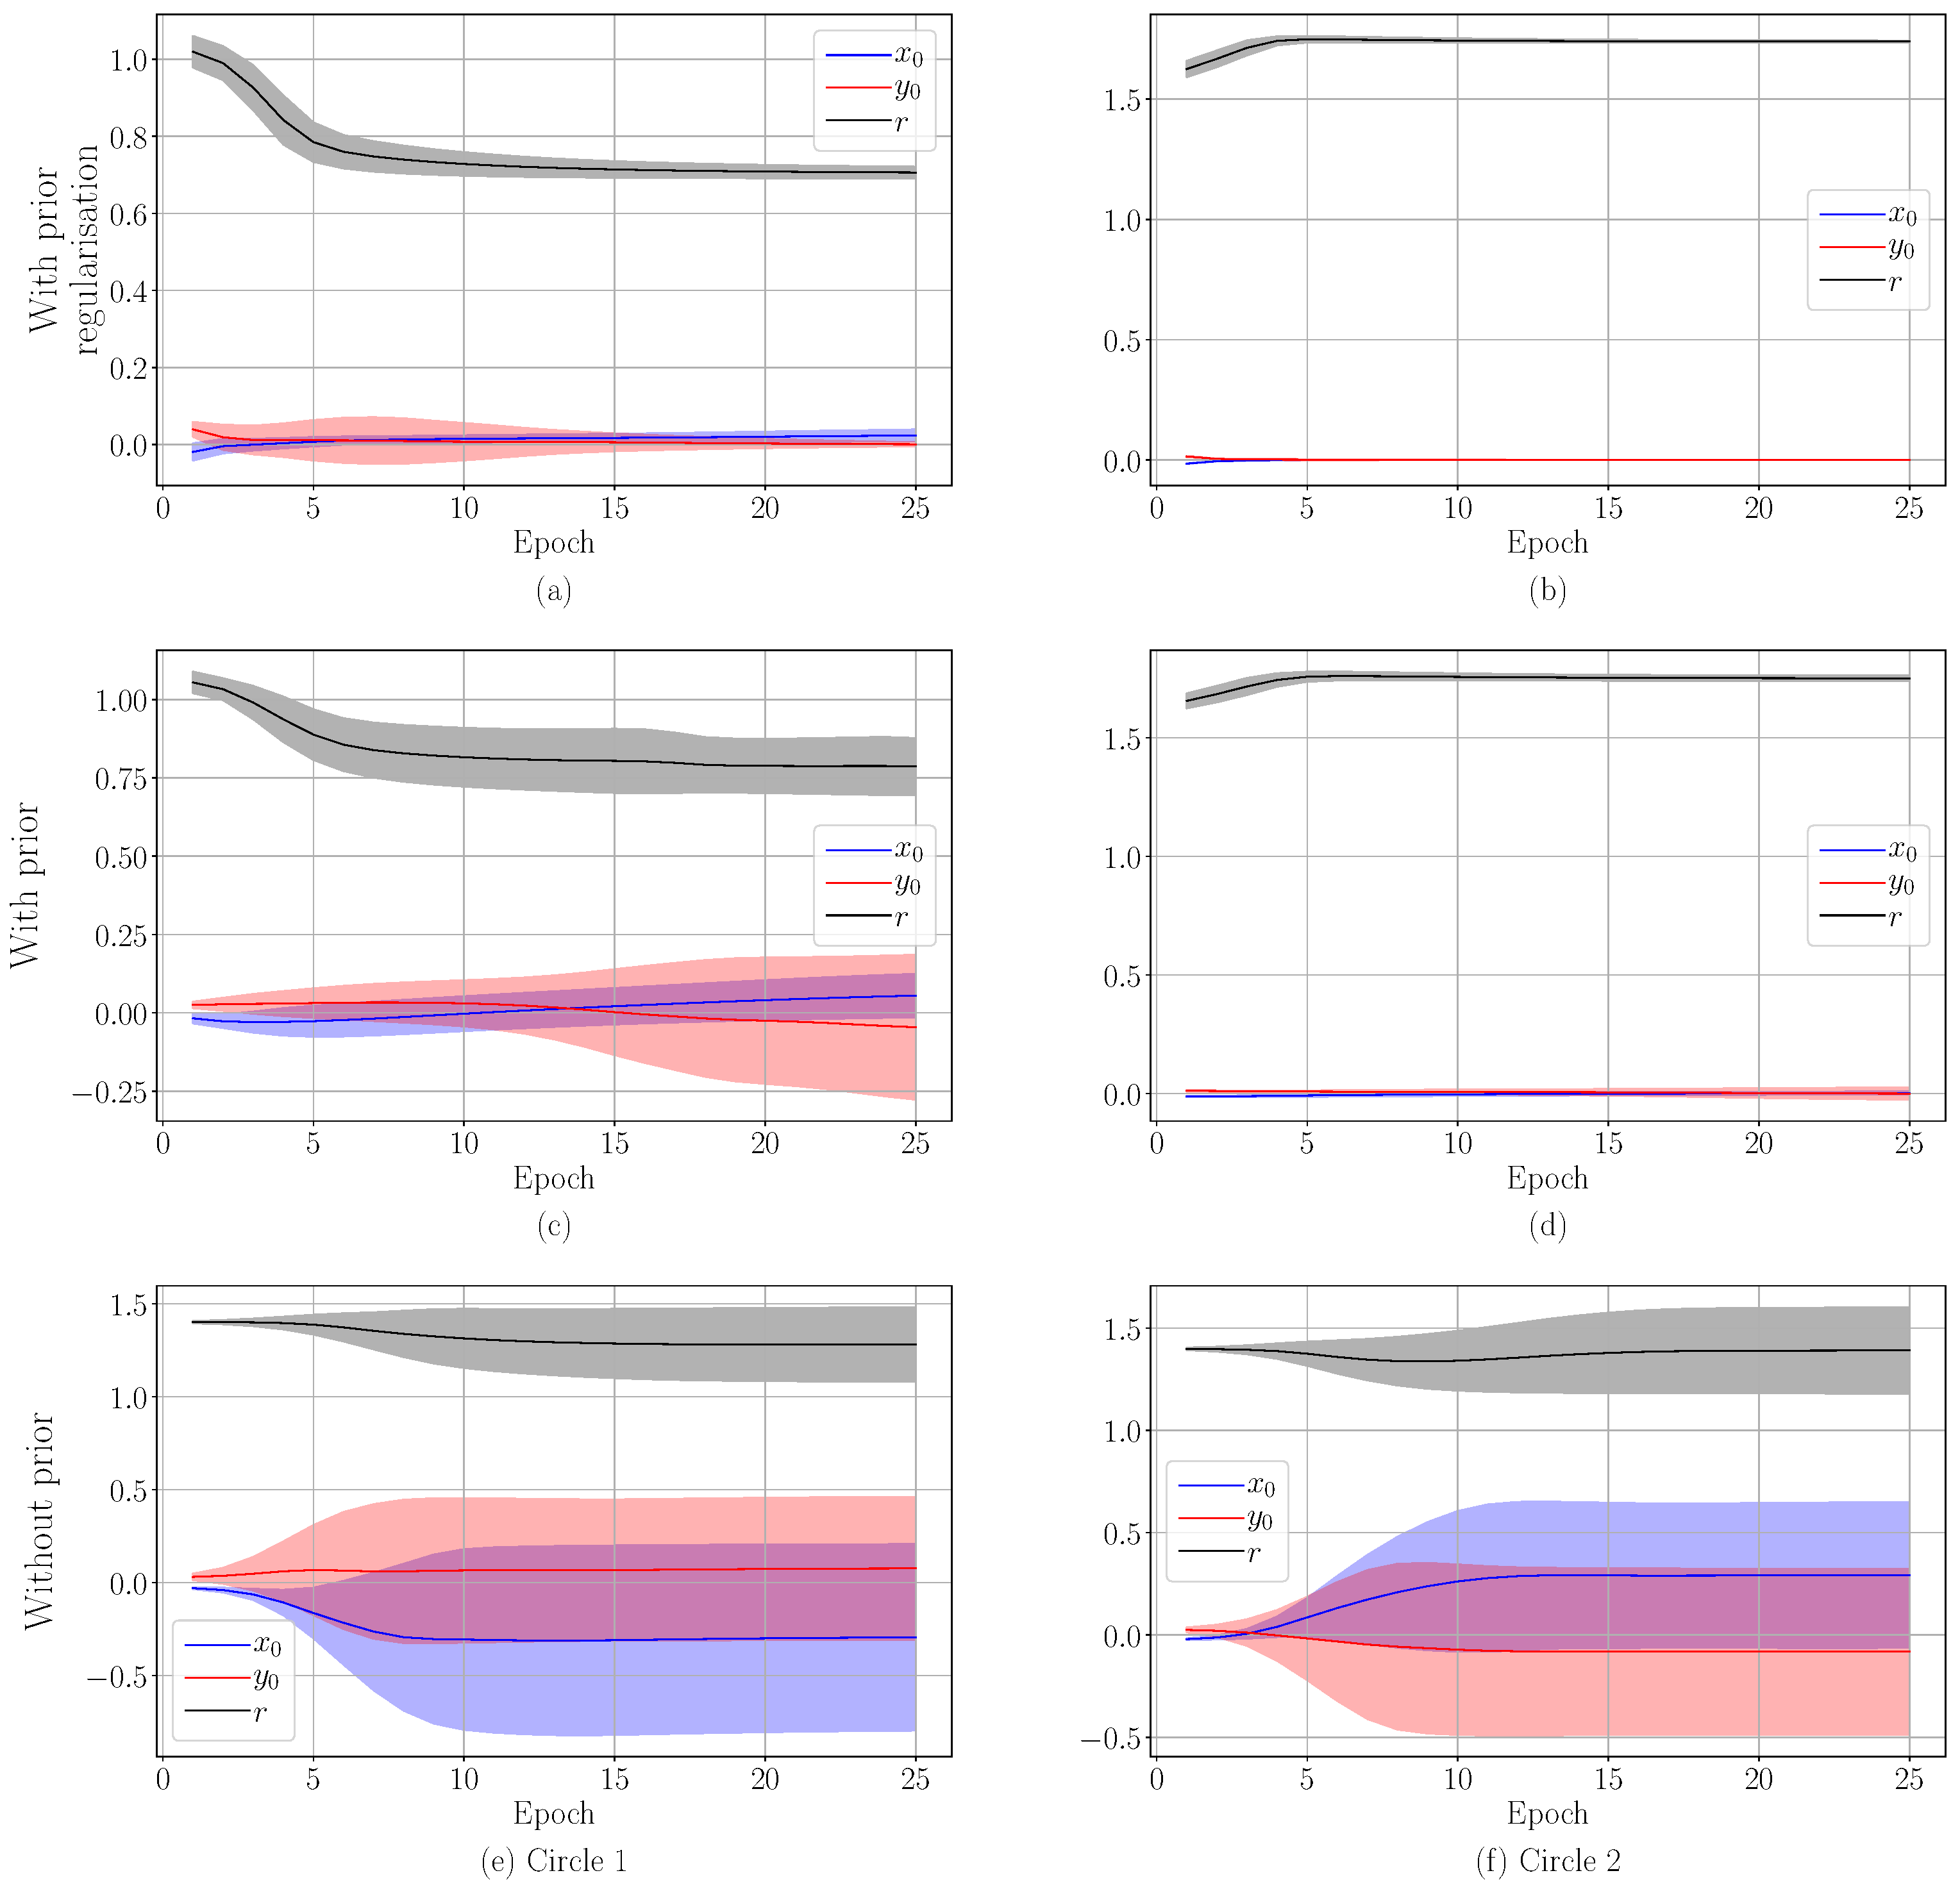
\includegraphics[width=1\textwidth]{result_eng/experiment_synthetic_param_progress}
\caption{График зависимости центра и радиуса окружностей от номера итерации: (a)--(b) модель с регуляризацией априорных распределений; (c)--(d) модель с заданными априорными распределениями на параметры моделей; (e)--(f) модель без задания априорных распределений}
\label{experiment:st:2:1}
\end{figure}

\begin{figure}[h!t]\center
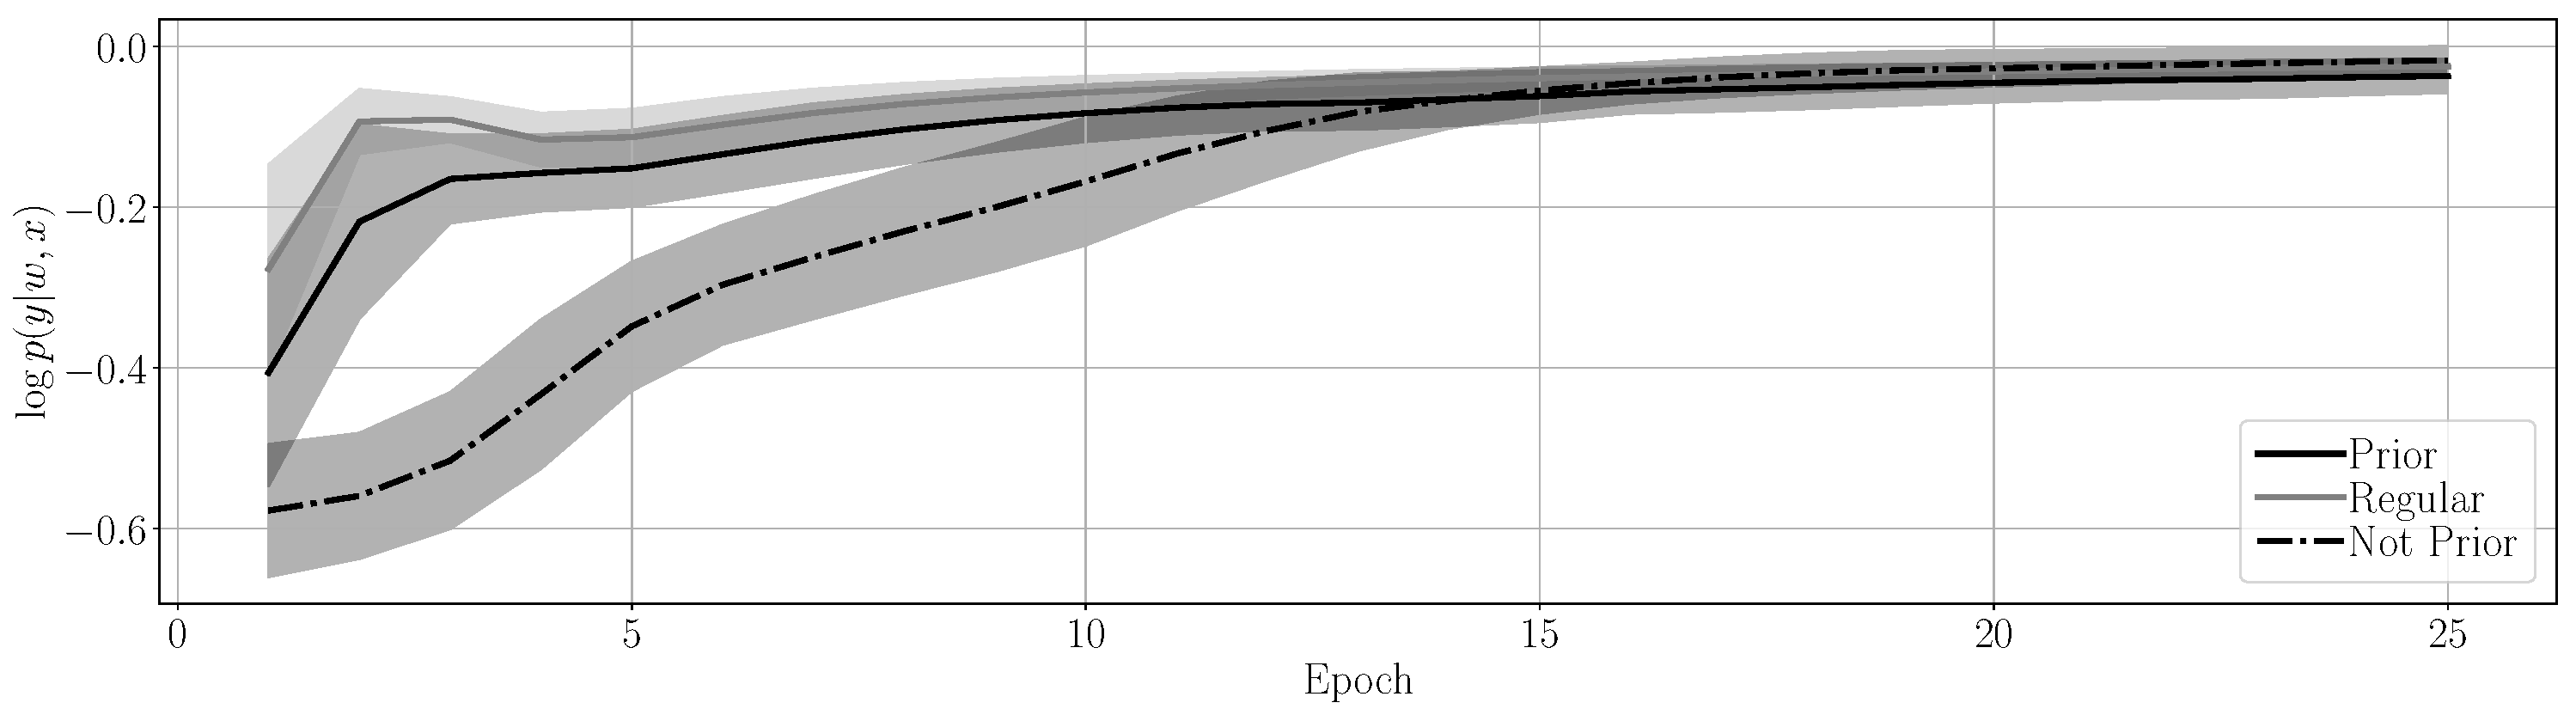
\includegraphics[width=1\textwidth]{result_eng/experiment_synt_likelihood_progress}
\caption{График зависимости логарифма правдоподобия модели от номера итерации ЕМ-алгорима}
\label{experiment:st:2:2}
\end{figure}

\begin{figure}[h!t]\center
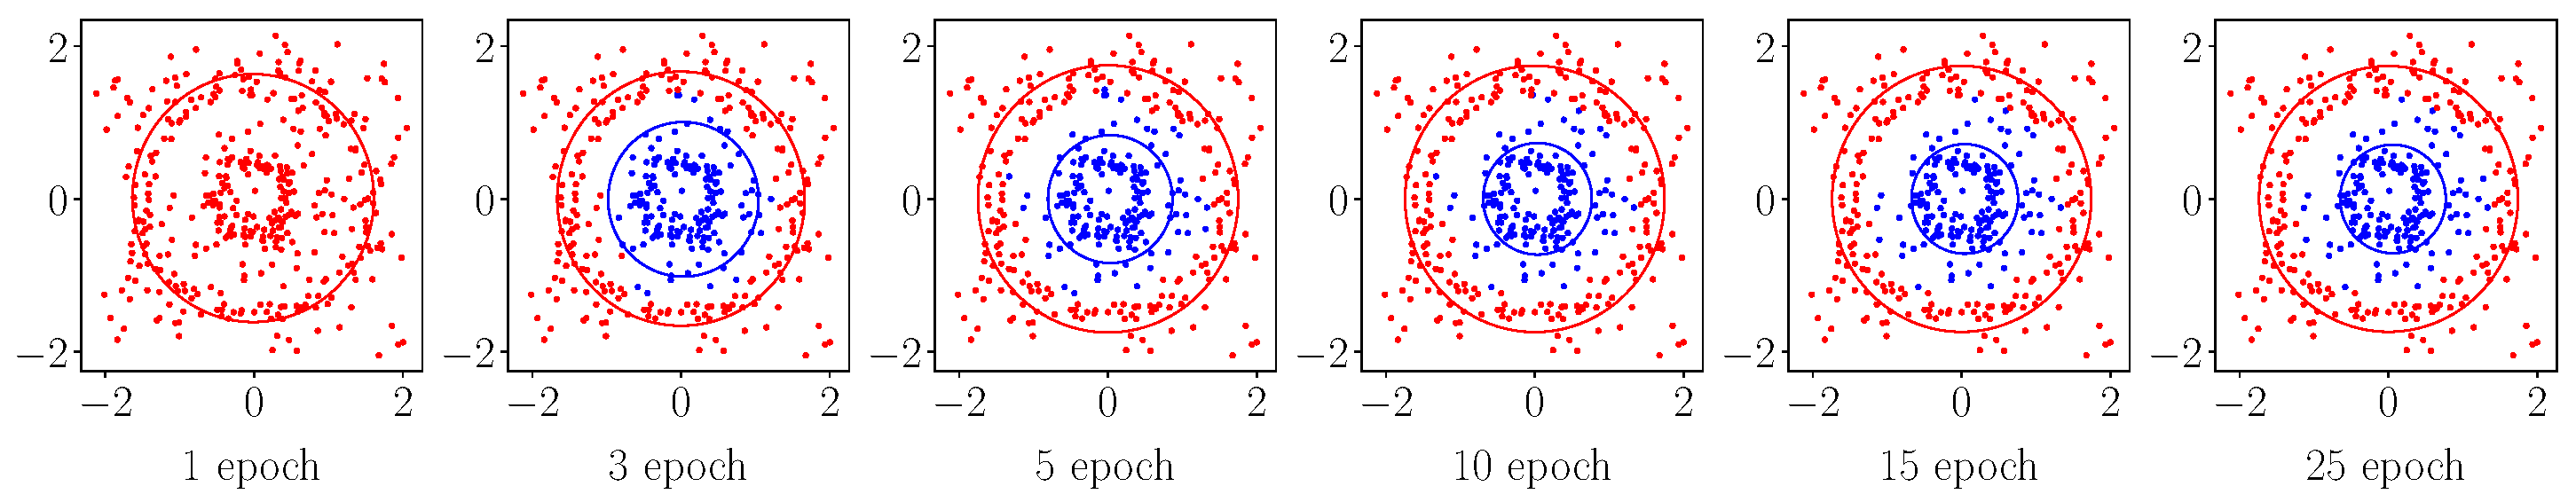
\includegraphics[width=1\textwidth]{result_eng/experiment_synt_regular_progress}
\caption{Визуализация процесса обучения для мультимодели с заданной регуляризацией: от 1й итерации до  25й итерации}
\label{experiment:st:2:3}
\end{figure}

\begin{figure}[h!t]\center
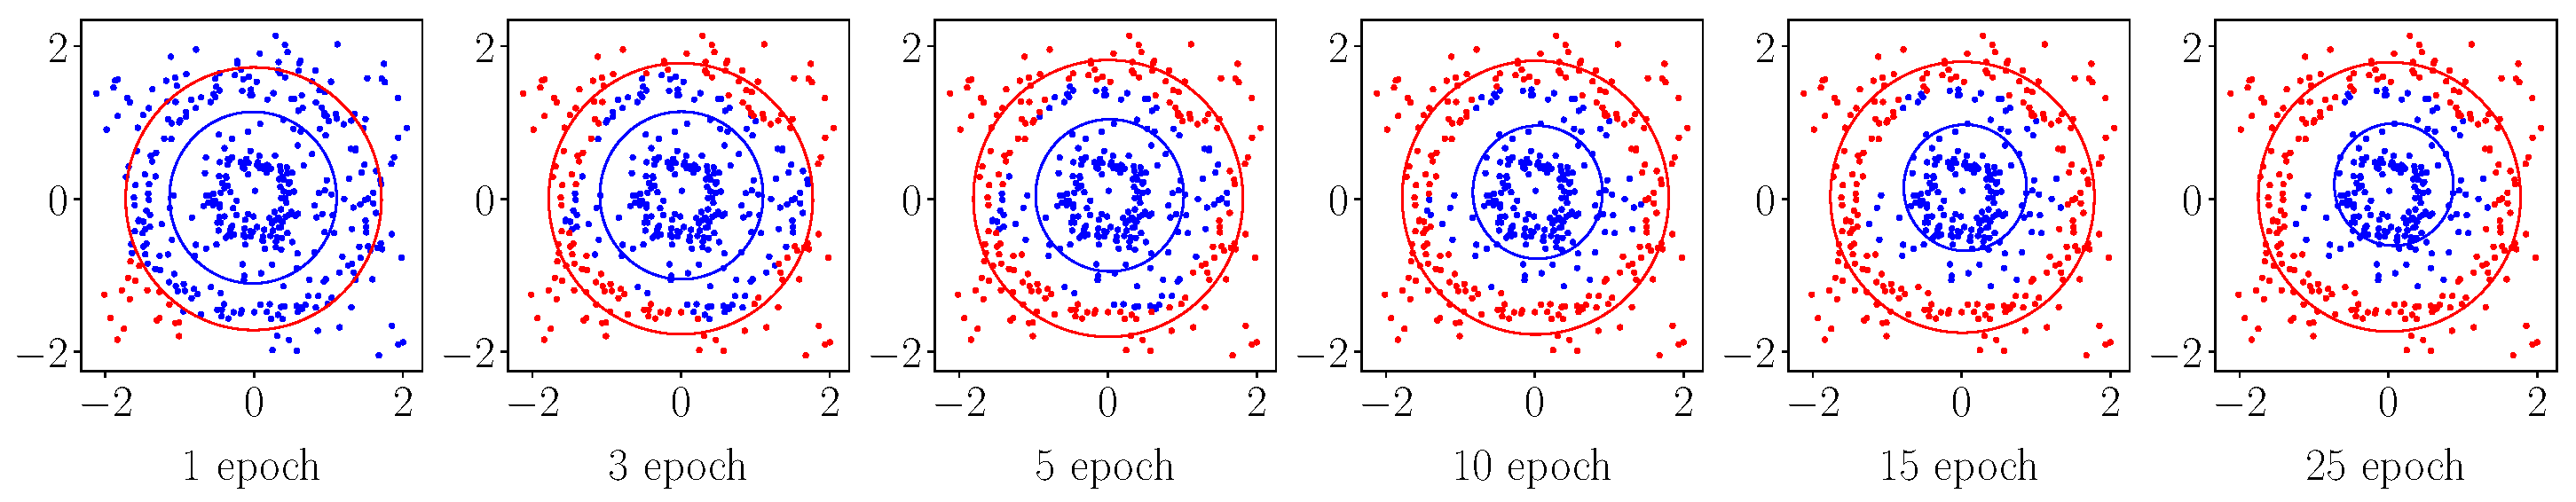
\includegraphics[width=1\textwidth]{result_eng/experiment_synt_prior_progress}
\caption{Визуализация процесса обучения для мультимодели с заданным априорным распределением на параметрах локальных моделей: от 1й итерации до 25й итерации}
\label{experiment:st:2:4}
\end{figure}

\begin{figure}[h!t]\center
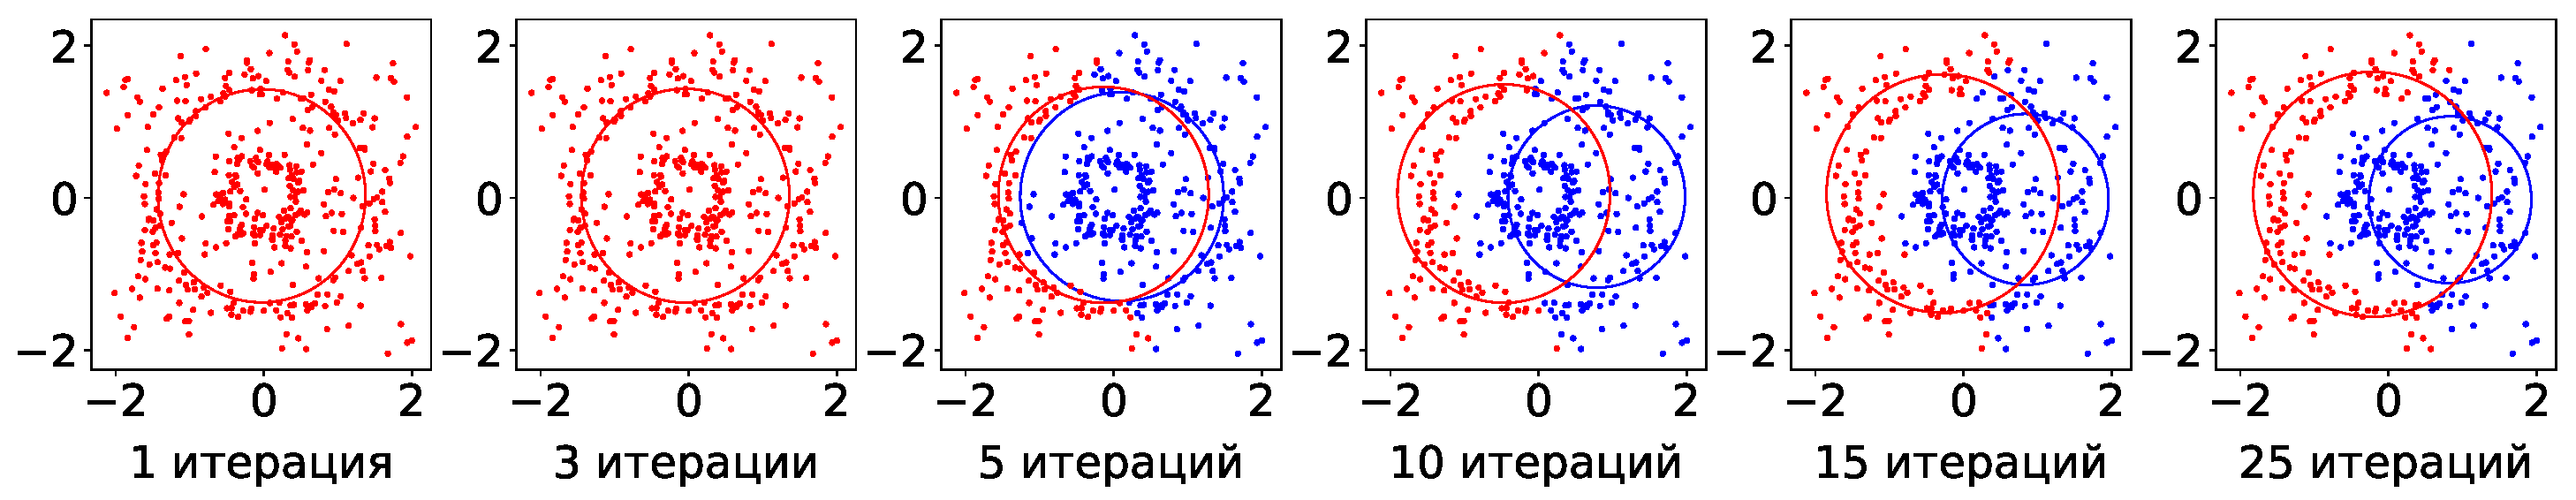
\includegraphics[width=1\textwidth]{result_eng/experiment_synt_not_prior_progress}
\caption{Визуализация процесса обучения для мультимодели баз заданных априорных распределений: от 1й итерации до 25й итерации}
\label{experiment:st:2:5}
\end{figure}
Для анализа свойств мультимоделей~$\mathfrak{M}_1, \mathfrak{M}_2, \mathfrak{M}_3$ во время обучения проведен вычислительный эксперимент. В качестве данных рассматривалась синтетическая выборка~Synthetic~3.

На рис.~\ref{experiment:st:2:1} показана зависимость радиуса и центра окружности от номера итерации. Мультимодель~$\mathfrak{M}_2$ с априорным распределением находит центры и радиусы окружностей в среднем лучше, чем мультимодель~$\mathfrak{M}_1$ без задания априорного распределения. Мультимодель~$\mathfrak{M}_3$ с заданием регуляризатора является более устойчивой, чем мультимодель~$\mathfrak{M}_2$, так как дисперсия восстановленных центров и радиуса окружностей меньше.

%Показано, что задание априорного распределения на модели улучшает качество предсказание центров и радиусов окружностей. Задание регуляризации априорных распределений улучшает устойчивость мультимодели, как видно на рис.~\ref{experiment:st:2:1} дисперсия параметров мультимодели с заданием регуляризации меньше чем дисперсия параметров других мультимоделей.
На рис.~\ref{experiment:st:2:2} показана зависимость правдоподобия мультимодели~\eqref{eq:ce:st:2:1} от номера итерации ЕМ--алгоритма. Правдоподобие модели на начальных этапах ЕМ--алгоритма растет быстрее в случае мультимоделей~$\mathfrak{M}_2, \mathfrak{M}_3$ чем в мультимодели~$\mathfrak{M}_1$. После 20-й итерации все три мультимодели имеют одинаковое правдоподобие.

На рис.~\ref{experiment:st:2:3}-\ref{experiment:st:2:5} показан процесс обучения смеси экспертов для разных мультимоделей. На рис.~\ref{experiment:st:2:5} проиллюстрирована работа ЕМ--алгоритма для мультимодели~$\mathfrak{M}_1$, которая не находит окружности верно. Иллюстрация работы ЕМ--алгоритма для мультимоделей~$\mathfrak{M}_2, \mathfrak{M}_3$ показана на рис.~\ref{experiment:st:2:3}-\ref{experiment:st:2:4}. Мультимодели $\mathfrak{M}_2, \mathfrak{M}_3$ находят обе окружности на изображении.

В ходе данного эксперимента показано, что задание априорных распределений улучшает качество мультимодели, позволяя находить нужные окружности в среднем лучше, чем мультимодель без заданого априорного распределения на параметрах локальных моделей. Задание регуляризации априорных распределений позволяет улучшить устойчивость мультимодели, так как дисперсия центра и радиуса окружностей становится меньше.
Также в эксперименте показано, что не смотря на примерное равенство правдоподобий~\eqref{experiment:st:2:2} различных мультимоделей, качество предсказание окружностей для разных мультимоделей существенно различается. В случае задания априорного распределения качество нахождения окружностей выше.

\paragraph{Анализ мультимоделей в зависимости от уровня шума.} 
\begin{figure}[h!t]\center
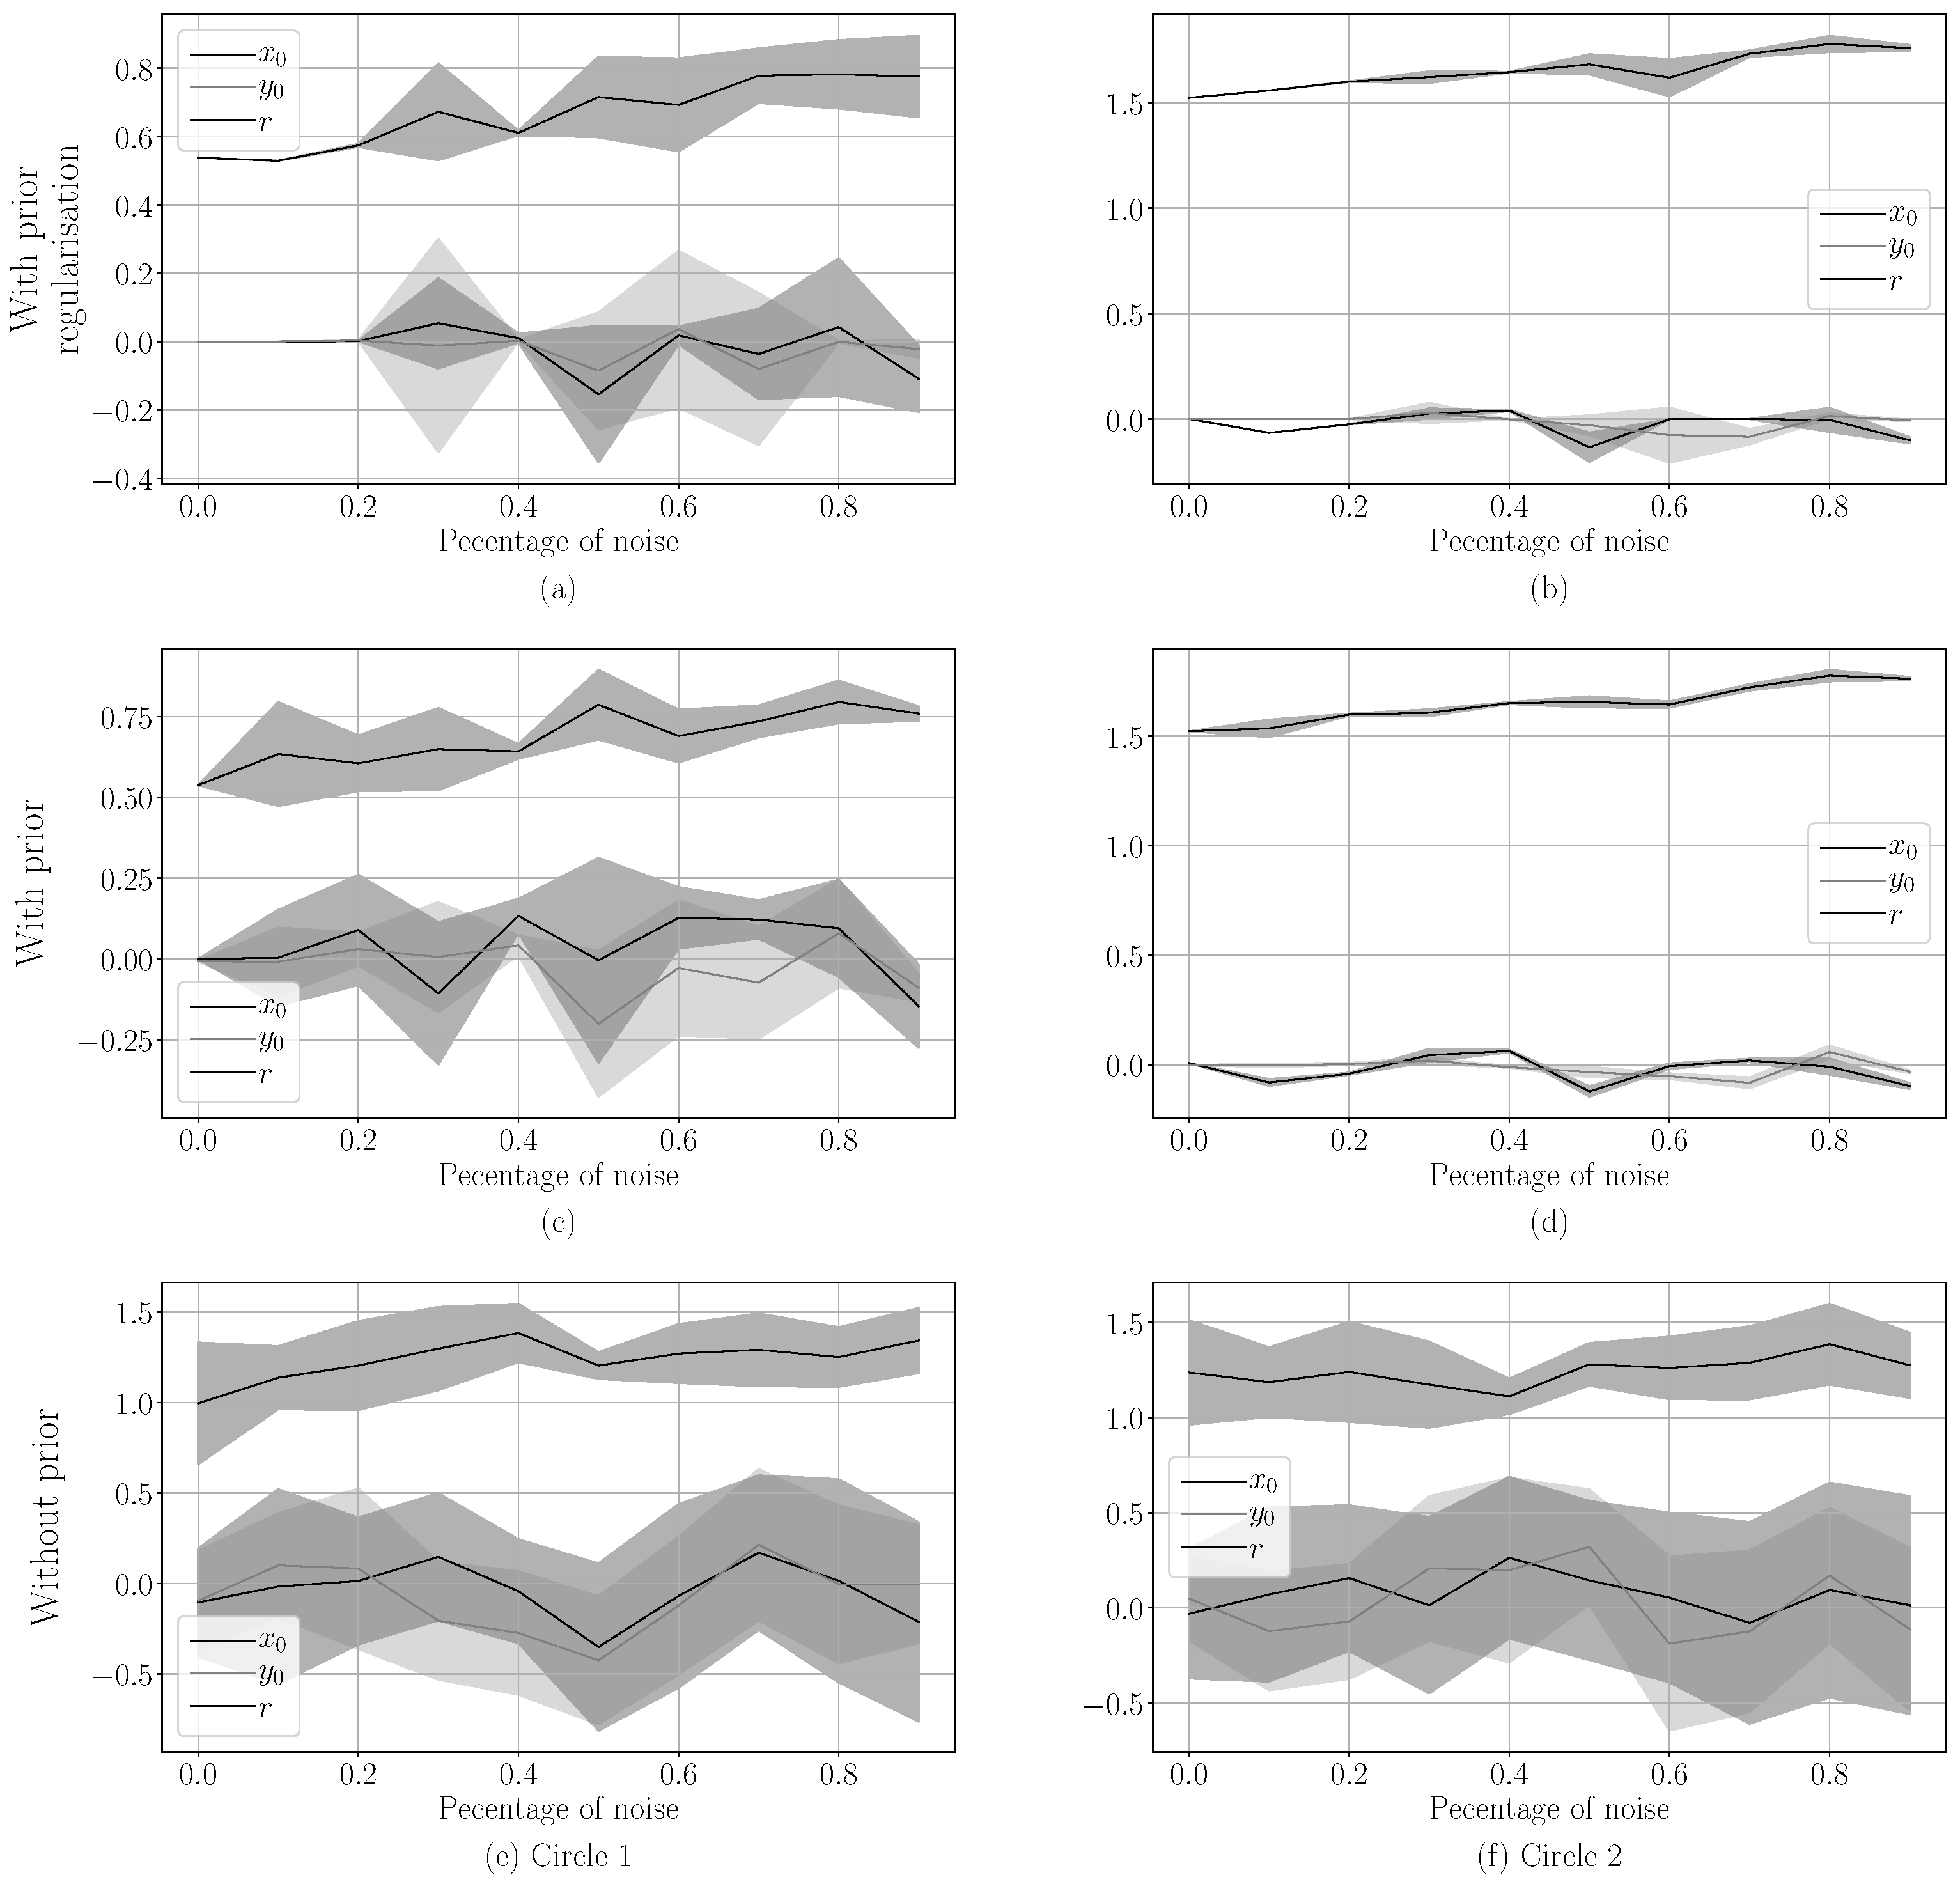
\includegraphics[width=1\textwidth]{result_eng/experiment_synthetic_param_progress_noise}
\caption{График зависимости центра и радиуса окружностей от номера итерации: (a)--(b) модель с регуляризацией априорных распределений; (c)--(d) модель с заданными априорными распределениями на параметры моделей; (e)--(f) модель без задания априорных распределений}
\label{experiment:st:3:1}
\end{figure}

\begin{figure}[h!t]\center
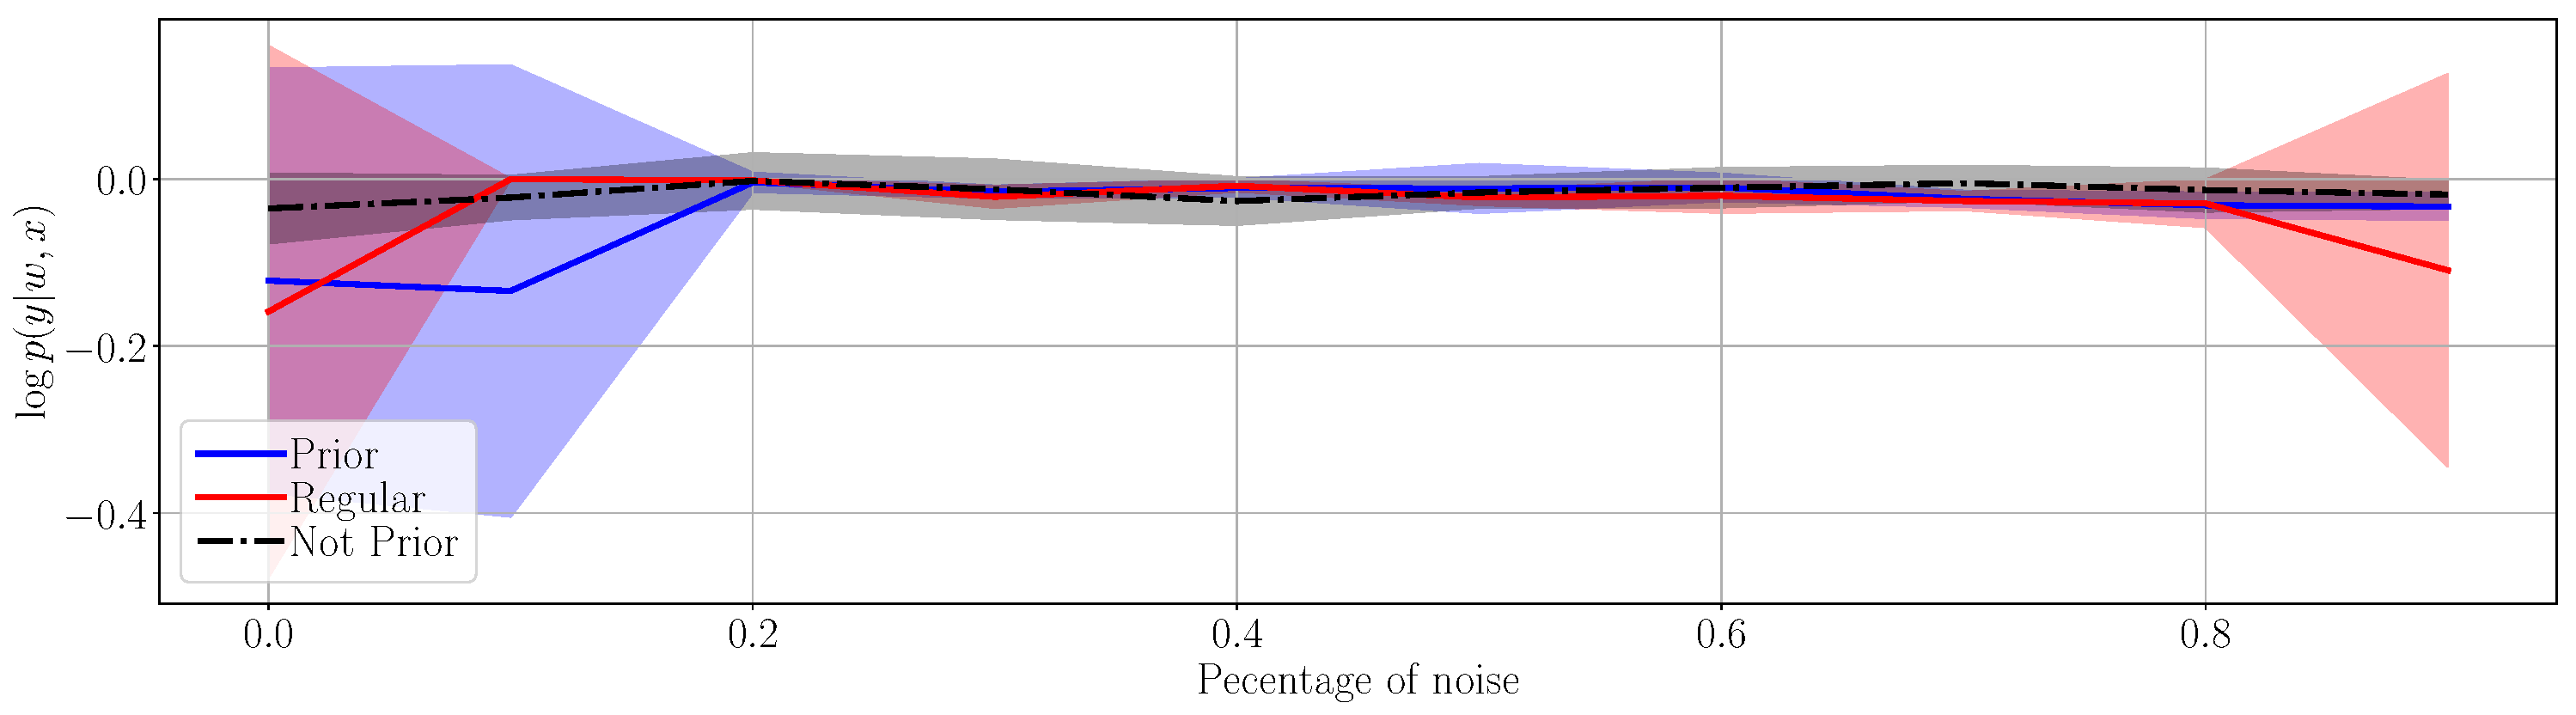
\includegraphics[width=1\textwidth]{result_eng/experiment_synt_likelihood_progress_noise}
\caption{График зависимости логарифма правдоподобия от уровня шума}
\label{experiment:st:3:2}
\end{figure}

Проведен вычислительный эксперимент, для анализа свойств мультимоделей~$\mathfrak{M}_1, \mathfrak{M}_2, \mathfrak{M}_3$ от уровня зашумленности. В качестве данных рассматривалась синтетическая выборка~Synthetic~1 с добавлением к ней разного уровня шума. Минимальный уровень шума равен $0$, когда нету шумовых точек, а максимальный уровень шума равен $1$, когда число шумовых точек равно числу точек обоих окружностей.

На рис.~\ref{experiment:st:3:1} показан график зависимости центра~$(x_{0}, y_{0})$ и радиуса~$r$ окружностей от уровня шума. Видно, что радиус окружностей растет при увеличении уровня шума. Центры окружностей модели~$\mathfrak{M}_2, \mathfrak{M}_3$ в среднем находят верно, но модель с регуляризацией~$\mathfrak{M}_3$ имеет меньшую дисперсию. Модель~$\mathfrak{M}_1$ имеет худший результат, так как имеет большую дисперсию по всем элементам: $x_0, y_0, r$.

На рис.~\ref{experiment:st:3:2} показан график зависимости логарифма правдоподобия модели~\eqref{eq:ce:st:2:1}. Видно, что все модели имеют одинаковое правдоподобие модели, но как показано на рис.~\ref{experiment:st:3:1} качество предсказание окружностей у разных моделей различается.

В данной части эксперимента показано, что наиболее устойчивой является модель~$\mathfrak{M}_3$ с регуляризацией априорных распределений.

\paragraph{Реальные данные.}
\begin{figure}[h!t]\center
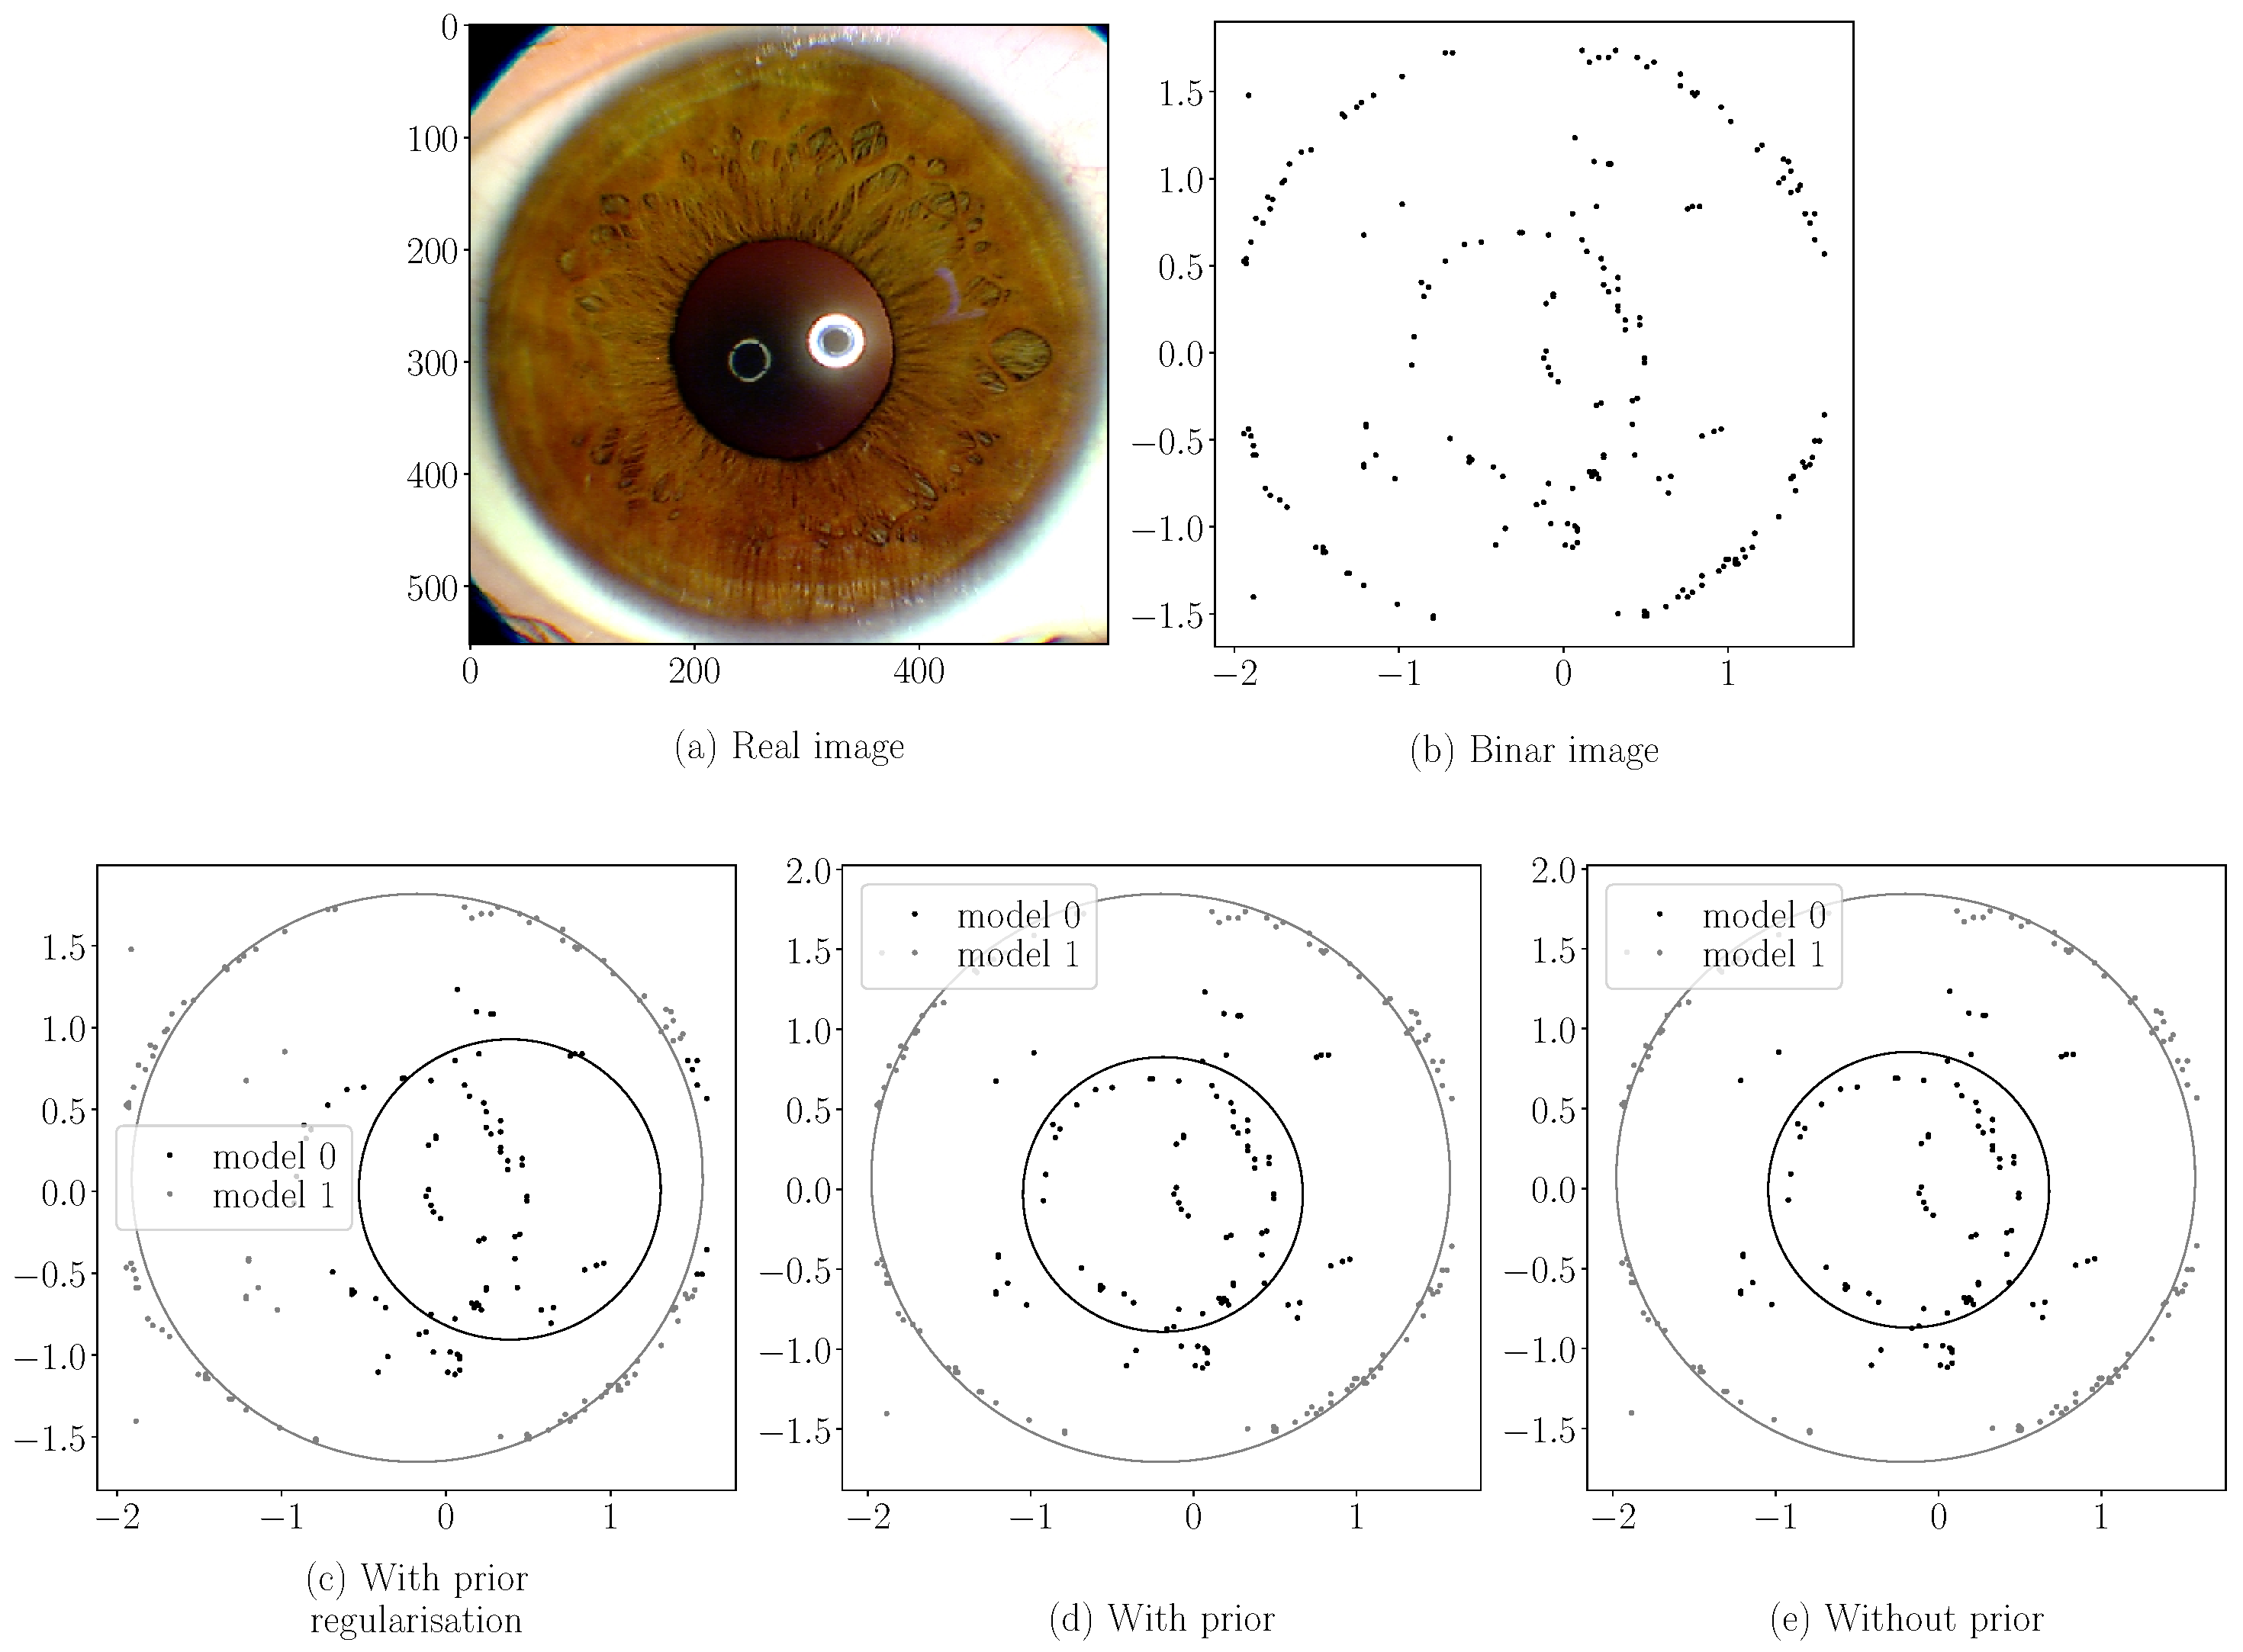
\includegraphics[width=0.9\textwidth]{result_eng/experiment_real_compare}
\caption{Мультимодель в зависимости от разных априорных предположений на реальном изображении: (a) исходное изображение; (b) бинаризованое изображение; (c) мультимодель без априорных предположений; (d) мультимодель с априорными распределениями на параметрах локальных моделей; (e) мультимодель с регуляризаций на априорных распределениях параметров локальных моделей}
\label{experiment:2}
\end{figure}

Проведен эксперимент на реальной выборке. В качестве данных рассматривались глаза, а точнее их предобработаное бинарное изображение с выделенными границами радужки и роговицы. Проводится анализ качества предсказания моделей~$\mathfrak{M}_1, \mathfrak{M}_2, \mathfrak{M}_3$.

На рис.~\ref{experiment:2} показан результат работы разных мультимоделей. Мультимодель~$\mathfrak{M}_1$ не верно находит меньшую окружность. Мультимодели~$\mathfrak{M}_2, \mathfrak{M}_3$ одинаково хорошо находят обе окружности.

%В случае, когда априорные распределения не заданы мультимодель верно находит внешнюю окружность, но не находит внутреннюю окружность. В случае, когда задано априорное распределение на параметры локальных моделей качество нахождение окружностей улучшилось, но внутренняя окружность все еще найдена не верно. После добавления к заданным априорным распределениям параметров регуляризации качество мультимодели выросло, что позволило верно найти и внутреннюю окружность.

\begin{figure}[h!t]\center
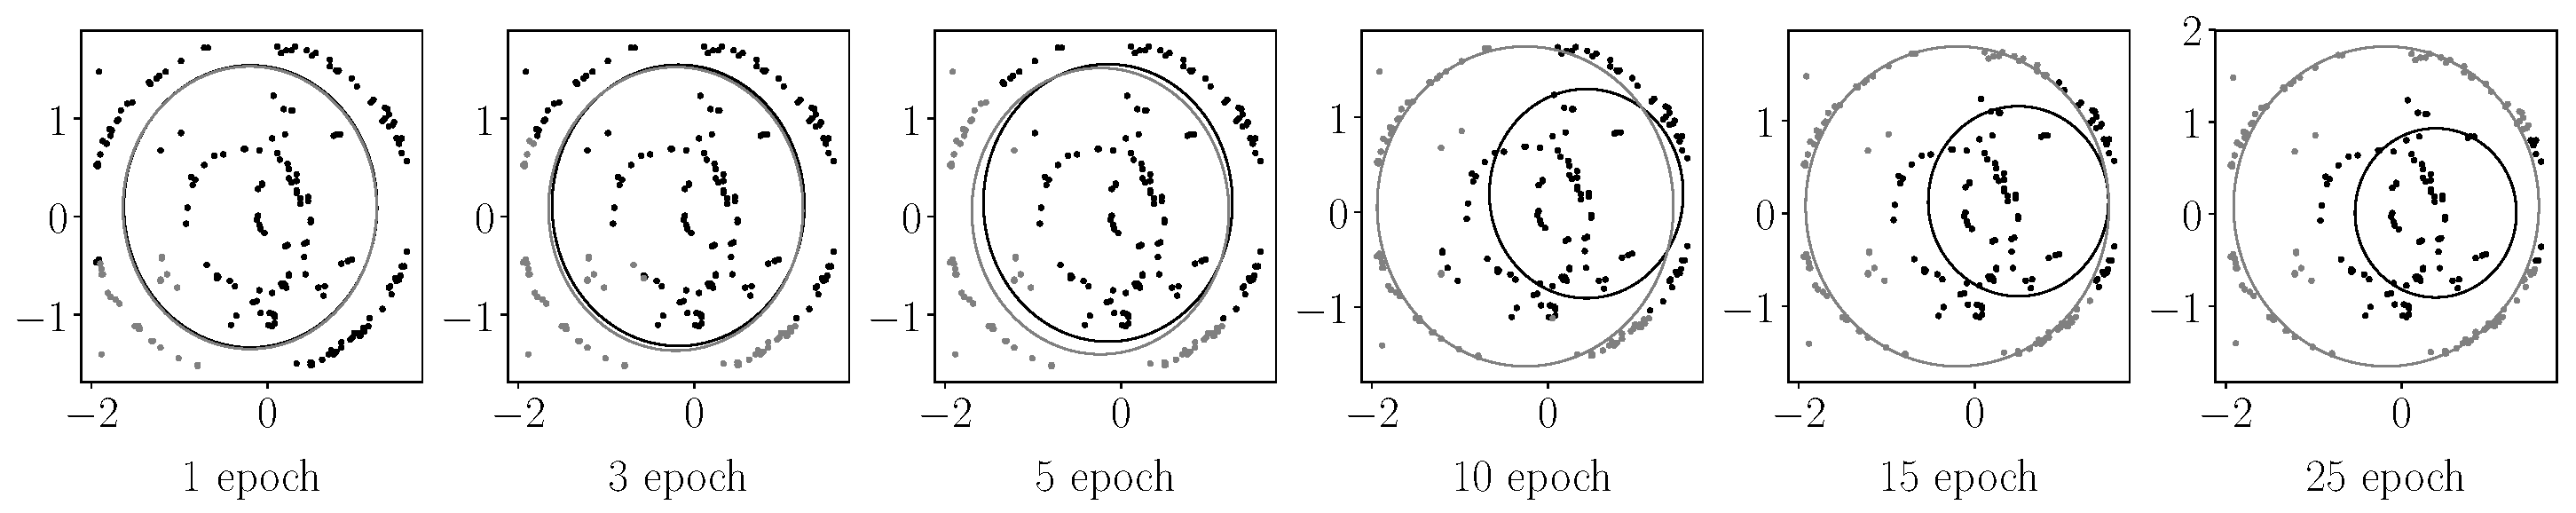
\includegraphics[width=1\textwidth]{result_eng/experiment_real_not_prior}
\caption{Визуализация процесса обучения для мультимодели без априорных предположений: от 1й итерации до 15й итерации}
\label{experiment:3}
\end{figure}

\begin{figure}[h!t]\center
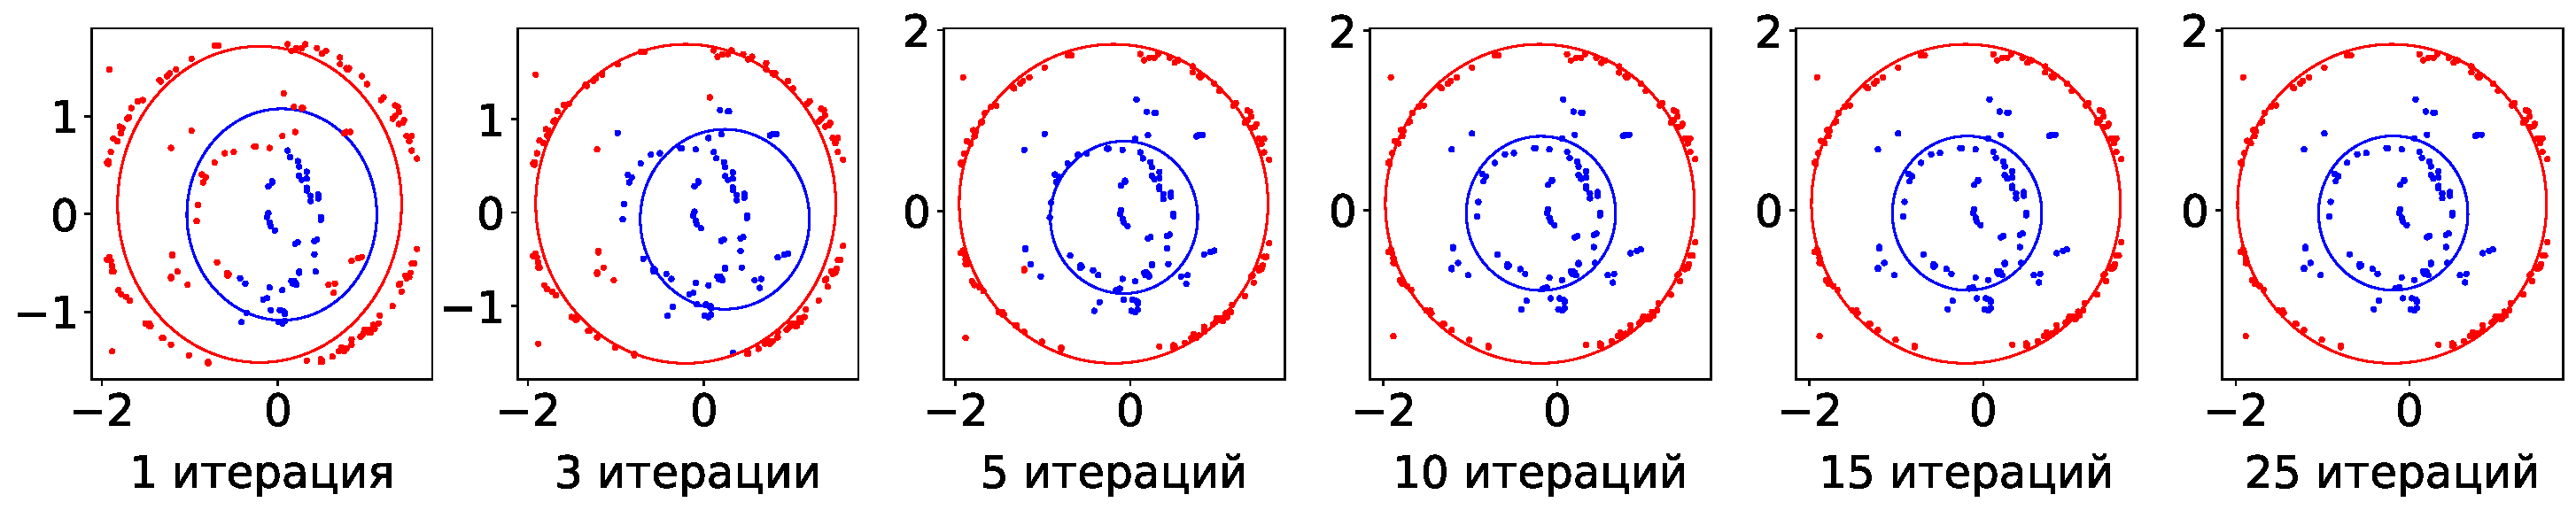
\includegraphics[width=1\textwidth]{result_eng/experiment_real_prior}
\caption{Визуализация процесса обучения для мультимодели с априорным распределением на параметрах локальных моделей: от 1й итерации до 15й итерации}
\label{experiment:4}
\end{figure}

\begin{figure}[h!t]\center
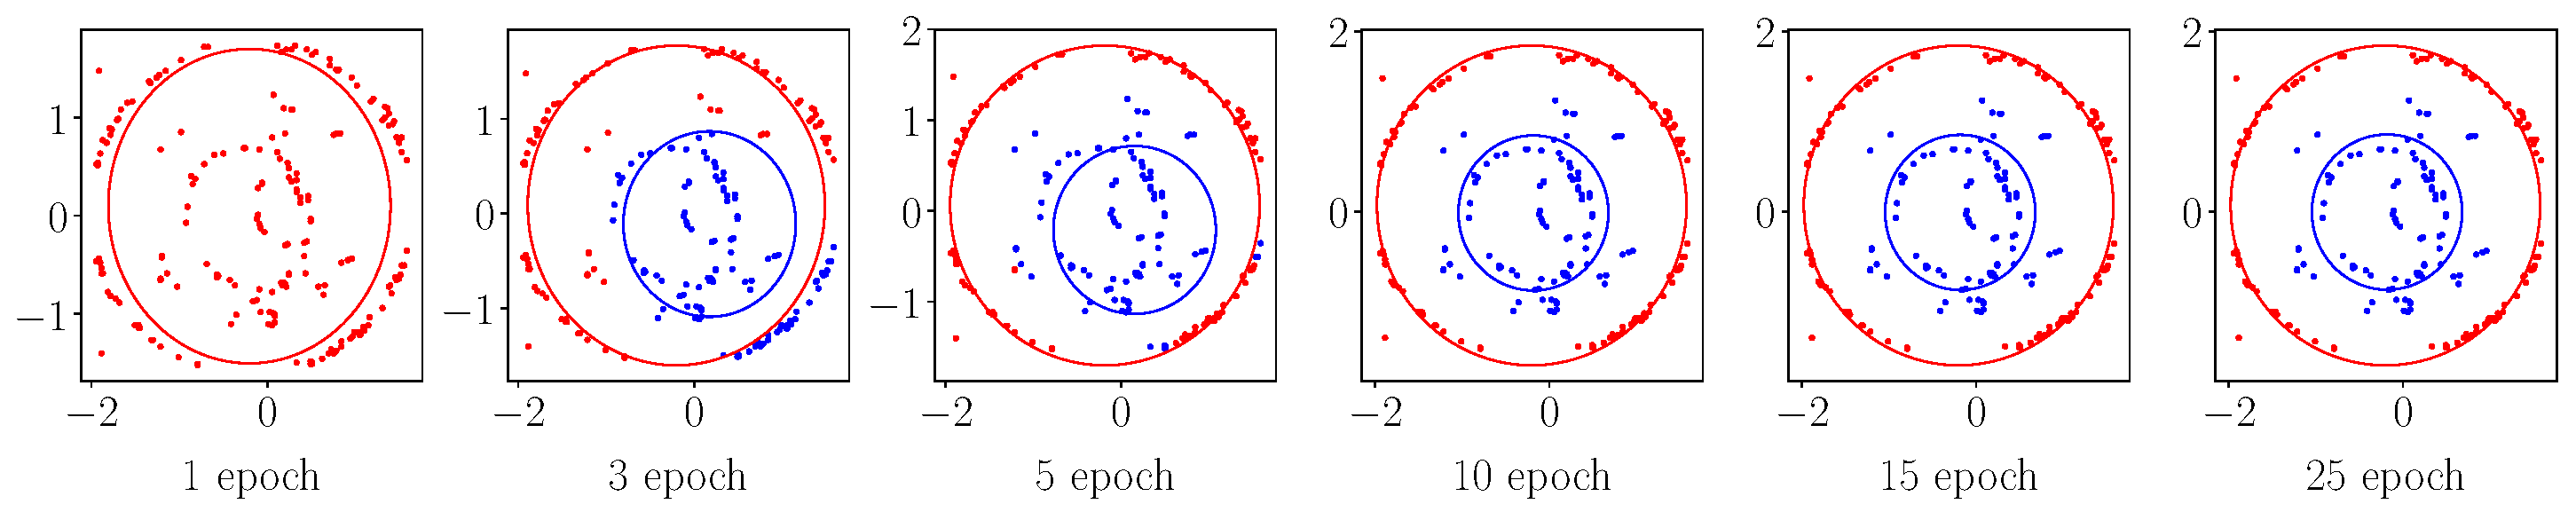
\includegraphics[width=1\textwidth]{result_eng/experiment_real_regular}
\caption{Визуализация процесса обучения для мультимодели с заданной регуляризацией: от 1й итерации до 15й итерации}
\label{experiment:5}
\end{figure}

На рис.~\ref{experiment:3}-\ref{experiment:5} показан процесс оптимизации мультимоделей. Показано изменение предсказания окружностей мультимоделями в процессе обучения. На рис.~\ref{experiment:3} показан процесс оптимизации параметров для мультимодели~$\mathfrak{M}_1$ без априорных знаний. На рис.~\ref{experiment:4} показан процесс оптимизации параметров для мультимодели~$\mathfrak{M}_2$, в которой задано априорное распределение на параметры локальных моделей. На рис.~\ref{experiment:5} показан процесс оптимизации параметров для мультимодели~$\mathfrak{M}_3$ с регуляризацией априорных распределений на параметрах локальных моделей.

В данной части эксперимента показано, что на реальных данных мультимодели~$\mathfrak{M}_2, \mathfrak{M}_3$ с заданными априорными распределениями и регуляризацией являются более точными в определении окружностей чем мультимодель~$\mathfrak{M}_2$ без априорных распределений.

\end{comment}
\section{Conclusion}
\begin{comment}
В данной работе проведено сравнение мультимоделей при различных априорных распределениях параметров локальной модели смеси и в случае, когда априорного распределения не было задано. В качестве данных использовались изображения концентрических окружностей с разным уровнем шума. Для поиска окружностей использовались линейные модели. В качестве шлюзовой функции использовалась двухслойная нейросеть.

Как показано в эксперименте, в случае, когда введены априорные знания на линейные модели, мультимодель является более точной, так как вернее находит окружности на изображениях.

Также был проведен эксперимент по исследованию различных способов регуляризации априорных распределений параметров локальных моделей. В эксперименте показано, что в случае, когда регуляризация задана, мультимодель находит окружности более устойчиво.

В ходе эксперимента было показано, что модели, которыу рассматриваются в работе, является чувствительными к выбросам. Для решения данной проблемы предлагается рассматривать не только локальные модели, которые описывают окружности, но также и модели, которые описывают шум. 

В дальнейшем планируется улучшить мультимодель при помощи задания априорного распределения на шлюзовую функцию. Планируется рассмотреть в качестве моделей не только модели, которые описывают данные, а также модель, которая отвечает за шум в данных. Предполагается, что вероятность шума мала, поэтому важно задать априорного распределение, которое учитывало бы этот факт.

\end{comment}

\begin{thebibliography}{99}
\bibitem{Tianqi2016}
	\textit{Chen Tianqi, Guestrin Carlos} XGBoost: A Scalable Tree Boosting System~// KDD ’16 Proceedings of the 22nd ACM SIGKDD International Conference on Knowledge Discovery and Data Mining. 2016.
	
\bibitem{Ishwaran2012}
	\textit{Chen Xi, Ishwaran Hemant} Random Forests for Genomic Data Analysis~// Genomics. 2012. Issues. 99, No 6. pp. 323--329.

\bibitem{Yuksel2012}
	\textit{Yuksel Seniha Esen, Wilson Joseph N., Gader Paul D} Twenty Years of Mixture of Experts~// IEEE Transactions on Neural Networks and Learning Systems. 2012. Issues. 23, No 8. pp. 1177--1193.

\bibitem{Shazeer2017}
	\textit{Noam Shazeer, Azalia Mirhoseini, Krzysztof Maziarz} Outrageously large neural networks: the sparsely-gated mixture-of-experts layer~// ICLR, 2017.

\bibitem{Edward2002}
	\textit{Rasmussen Carl Edward, Ghahramani Zoubin} Infinite Mixtures of Gaussian Process Experts~// Advances in Neural Information Processing Systems 14. 2002. pp. 881–888.
	
\bibitem{Jordan1994}
	\textit{M.~I.~Jordan} Hierarchical mixtures of experts and the EM algorithm~// Neural Comput., vol. 6, no. 2, pp. 181–214, 1994.
	
\bibitem{Lima2007}
	\textit{C.~A.~M.~Lima, A.~L.~V. Coelho, F.~J.~Von~Zuben} Hybridizing mixtures of experts with support vector machines: Investigation into nonlinear dynamic systems identification~// Inf. Sci., vol. 177, no. 10, pp. 2049–2074, 2007.

\bibitem{Cao2003}
	\textit{L.~Cao} Support vector machines experts for time series forecasting~// Neurocomputing, vol. 51, pp. 321–339, Apr. 2003.

\bibitem{Dempster1977}
	\textit{A. P. Dempster, N. M. Laird and D. B. Rubin} Maximum Likelihood from Incomplete Data via the EM Algorithm~// Journal of the Royal Statistical Society. Series B (Methodological), Vol. 39, No. 1 pp. 1-38, 1977.
	
\bibitem{Jordan1991}
	\textit{M.~I.~Jordan, R.~A.~Jacobs} Hierarchies of adaptive experts~// in Advances in Neural Information Processing Systems. Cambridge, MA: MIT Press, 1991, pp. 985–992.
	
\bibitem{Yumlu2003}
	\textit{M.\,S.~Yumlu, F.\,S.~Gurgen,  N.~Okay} Financial time series prediction using mixture of experts~// in Proc. 18th Int. Symp. Comput. Inf. Sci., 2003, pp. 553--560.
	
\bibitem{Cheung1995}
	\textit{Y.~M.~Cheung, W.~M.~Leung, and L. Xu} Application of mixture of experts model to financial time series forecasting~// in Proc. Int. Conf. Neural Netw. Signal Process., 1995, pp. 1--4.
	
\bibitem{Weigend2000}
	\textit{A. S. Weigend, S. Shi} Predicting daily probability distributions of S\&P500 returns~// J. Forecast., vol. 19, no. 4, pp. 375--392, 2000.
	
\bibitem{Ebrahimpour2009}
	\textit{R. Ebrahimpour, M. R. Moradian, A. Esmkhani, F. M. Jafarlou} Recognition of Persian handwritten digits using characterization loci and mixture of experts~// J. Digital Content Technol. Appl., vol. 3, no. 3, pp. 42–46, 2009.
	
\bibitem{Estabrooks2001}
	\textit{A.~Estabrooks, N.~Japkowicz} A mixture-of-experts framework for text classification~//in Proc. Workshop Comput. Natural Lang. Learn., Assoc. Comput. Linguist., 2001, pp. 1--8.
	
\bibitem{Mossavat2010}
	\textit{S. Mossavat, O. Amft, B. de Vries, P. Petkov, W. Kleijn} A Bayesian hierarchical mixture of experts approach to estimate speech quality~// in Proc. 2nd Int. Workshop Qual. Multimedia Exper., pp. 200--205., 2010

\bibitem{Peng1996}
	\textit{F. Peng, R. A. Jacobs, M. A. Tanner} Bayesian inference in mixtures-of-experts and hierarchical mixtures-of-experts models with an application to speech recognition~// J. Amer. Stat. Assoc., vol. 91, no. 435, pp. 953–960, 1996.
	
\bibitem{Tuerk2001}
	\textit{A. Tuerk} The state based mixture of experts HMM with applications to the recognition of spontaneous speech~// Ph.D. thesis, Dept. Eng., Univ. Cambridge, Cambridge, U.K., 2001.
	
\bibitem{Sminchisescu2007}
	\textit{C. Sminchisescu, A. Kanaujia, and D. Metaxas} B M3 E: Discrimina- tive density propagation for visual tracking~// IEEE Trans. Pattern Anal. Mach. Intell., vol. 29, no. 11, pp. 2030–2044, 2007.

\bibitem{Matveev2010}
	\textit{I. Matveev} Detection of iris in image by interrelated maxima of brightness gradient projections~// Appl.Comput. Math. 9 (2), 252–257, 2010.

\bibitem{Matveev2014}
	\textit{I. Matveev, I. Simonenko}. Detecting precise iris boundaries by circular shortest path method~// Pattern Recognition and Image Analysis. 24. 304-309. 2014.
	
\bibitem{Bowyer2010}
	\textit{K. Bowyer, K. Hollingsworth, P. Flynn} A Survey of Iris Biometrics Research: 2008–2010.
	
\bibitem{bishop2006}
	\textit{Bishop C.} Pattern Recognition and Machine Learning.~---~Berlin: Springer, 2006. 758~p.

 \end{thebibliography}
 
 \appendix

\begin{comment}
\section{Постановка задачи нахождения параметров эллипса}\label{apendix:el}
Задано бинарное изображение:
\[
\label{apendix:el:eq:1}
\begin{aligned}
\textbf{M} \in \{0,1\}^{m_1 \times m_2},
\end{aligned}
\]
где $0$ отвечает черной точке --- изображения, $1$ --- белой точке фона.

По изображению $\textbf{M}$ строится выборка $\textbf{C}$, элементами которой являются координаты~$x_i, y_i$ белых точек на картинке:
\[
\label{apendix:el:eq:2}
\begin{aligned}
\textbf{C} \in  \mathbb{R}^{N \times 2},
\end{aligned}
\]
где $N$ --- число черных точек на изображении $\textbf{M}$.

Обозначим $x_0, y_0$ --- центр эллипса, который требуется найти на бинарном изображении $\textbf{M}$, а $a, b$ его коэффициенты вдоль координат. Элементы выборки $\left(x_i, y_i\right)\in\textbf{C}$ являются геометрическим местом точек, которое заданно уравнением эллипса:
\[
\label{apendix:el:eq:3}
\begin{aligned}
\left(x_i - x_0\right)^{2}+\frac{a^2}{b^2}\left(y_i-y_0\right)^2 = a^2.
\end{aligned}
\]
Раскрыв скобки получим уравнение
\[
\label{apendix:el:eq:4}
\begin{aligned}
\left(2x_0\right)\cdot x_i + \left(\frac{2y_0a^2}{b^2}\right)\cdot y_i + \left(-\frac{a^2}{b^2}\right)y_{i}^{2} + \left(a^2-x_0^2-\frac{a^2}{b^2}y_0^2\right)\cdot1 = x_{i}^2.
\end{aligned}
\]
Получаем задачу линейной регрессии для нахождения параметров окружности:
\[
\label{apendix:el:eq:5}
\begin{aligned}
\textbf{X}\textbf{w} \approx \textbf{y},  \quad \textbf{X} = \text{concat}\left[\textbf{C}, \left[y_1^2, y_2^2, \cdots, y_N^2\right]^{\mathsf{T}}, \textbf{1}\right], \quad \textbf{y} = [x_1^2, x_2^2, \cdots, x_N^2]^{\mathsf{T}},
\end{aligned}
\]
где найденые оптимальные параметры линейной регрессии $\textbf{w} = \bigr[w_1, w_2, w_3, w_4\bigr]^{\mathsf{T}}$ восстанавливают параметры окружности:
\[
\label{apendix:el:eq:6}
\begin{aligned}
x_0 = \frac{w_1}{2}, \quad y_0 = -\frac{w_2}{2w_3}, \quad a^2 = w_4-\frac{w_1}{2}-\frac{w_2^2}{4w_3}, \quad b^2 = -\frac{1}{w_3}\left(w_4-\frac{w_1}{2}-\frac{w_2^2}{4w_3}\right).
\end{aligned}
\]

Решение уравнения~\eqref{apendix:el:eq:5} находит параметры единственного эллипса на изображении.
\end{comment}

\end{document}

